\documentclass[11pt,a4paper]{article}

\usepackage[utf8]{inputenc}
\usepackage[T1]{fontenc}
\usepackage{amsmath,amssymb,mathtools}
\usepackage{geometry}
\usepackage{xcolor}
\usepackage{hyperref}
\usepackage{booktabs}
\usepackage{array}
\usepackage{enumitem}
\usepackage{graphicx}
\usepackage{tikz}

\geometry{margin=1in}
\setlist[itemize]{itemsep=0.2em,topsep=0.3em}
\setlist[enumerate]{itemsep=0.2em,topsep=0.3em}

\hypersetup{
  colorlinks=true,
  linkcolor=blue!50!black,
  citecolor=blue!50!black,
  urlcolor=blue!60!black,
  pdftitle={MaxwellFD: 2D Yee FDTD and FDFD},
  pdfauthor={Tom Smy}
}
\makeatletter
\g@addto@macro{\UrlBreaks}{\do\_\do\-}
\makeatother

\title{\textbf{MaxwellFD: 2D Yee FDTD and FDFD}\\[0.35em]
\large Physics, methods, and code}
\author{Tom Smy}
\date{29 September 2026}

\begin{document}
\maketitle

\begin{abstract}
MaxwellFD is a Python Yee-cell solver. One uniform Cartesian grid, one
material sampling, and one pair of discrete curls feed both a leapfrog
(FDTD) and a sparse frequency-domain system (FDFD). Phasors use
$e^{j\omega t}$, the same convention as MaxwellMOM. This note describes the
physics and the method that are actually coded, how the package is
organized, and how the Fresnel-slab, dielectric-cylinder, PML
line-current, and open PEC-cylinder examples are run and drawn. The
equation reference is \texttt{FD\_LaTeX\_Reference.tex}. The convolutional
PML from that note is coded as a stretch of the normal derivatives on a
PEC-backed band.
Embedded PEC and PMC objects remove Yee samples, and an open PEC cylinder
is compared with the Mie series on that band. An open dielectric cylinder
on the same band is driven by the contrast current
$J=j\omega(\varepsilon-\varepsilon_0)E_{\mathrm{inc}}$. A 3D PEC cavity
checks three pure modes of the Yee cell. An open dielectric sphere, on a
PML small enough to factor, is compared with the Mie series. A resistive
sheet adds its conductance to one Ampere cell and is compared with the
analytic reflection. A symmetric GSTC sheet replaces the magnetic sample
on one face and is compared the same way. A finite run of that face, with
$\chi_{ee}=\chi_{mm}=-2j/k$, is a normal-incidence absorber on a four-sided PML.
The normal magnetic susceptibility $\chi_{mm}^{nn}$ enters the TMz jump, and
one periodic cell at an angle is compared with the analytic reflection and
transmission. The same susceptibilities on a $10\lambda$ sheet at $30^\circ$
are the open scattered-field run.
\end{abstract}

\tableofcontents
\newpage

\section{Status}
\label{sec:status}

Version 0.1.0 contains the following.

\begin{enumerate}
\item The 2D cell in free space and in a uniform isotropic medium: TMz and
TEz curls, PEC and periodic walls, the CFL limit, cavity eigenvalues, a
manufactured FDFD solve, and a periodic standing wave.
\item Volumetric media. A staircase assigns a real $\varepsilon$, $\mu$, and
$\sigma\ge 0$ to each Yee sample. FDFD accepts a complex
$\varepsilon(\omega)$. FDTD adds one bulk Debye pole or one bulk Lorentz
pole through a polarization current. The closed-box checks are a Fresnel
slab and a dielectric cylinder, both driven by an analytic Dirichlet trace
on the existing PEC wall.
\item The convolutional PML on a PEC-backed band, for both polarizations
and both drivers. In FDFD every derivative carries the factor
$1/s_w(\omega)$. The leapfrog keeps one auxiliary for each of those
derivatives. A line current is compared with the outgoing Hankel function
on the unstretched samples.
\item Embedded PEC and PMC objects. PEC drops every electric sample inside
its region. PMC drops every magnetic sample. The open check is a PEC
cylinder: the unknown is the scattered field, the object carries the trace
$-E_{\mathrm{inc}}$, and the PML absorbs the outgoing wave.
\item An open dielectric cylinder on that PML. The staircase disk stays in
the operator. The incident wave is the impressed current
$J=j\omega(\varepsilon-\varepsilon_0)E_{\mathrm{inc}}$, and a free sample
of the total field is $E_s+E_{\mathrm{inc}}$.
\item The 3D Yee cell and a sparse FDFD operator on a rectangular box.
Uniform isotropic media, with PEC and periodic walls. Three pure cavity
modes are checked by a Rayleigh quotient against the semi-discrete
frequency with the third centered difference.
\item An open dielectric sphere. The 3D FDFD operator stretches a
PEC-backed PML and keeps a staircase ball in the permittivity. The
incident wave is the contrast current, the unknown is the scattered
field, and the total electric field is compared with the Mie series.
\item A $z$-directed Hertzian dipole. One $E_z$ sample carries
$J_z=I\ell/(\Delta x\Delta y\Delta z)$. The electric field outside the
PML, and at least $\lambda/4$ from the element, is compared with the
outgoing spherical wave.
\item A resistive sheet of normal $\hat{\mathbf{y}}$. The conductance
$1/(Z_s\Delta y)$ is added to $\sigma$ on the tangential electric samples
of the one Ampere cell that contains the sheet. The closed-box check
compares the packed electric field with the analytic reflection and
transmission.
\item A symmetric GSTC sheet of normal $\hat{\mathbf{y}}$. The magnetic
sample on one face is replaced by the pair $H^-$ and $H^+$. Tangential
$\chi_{ee}$ and $\chi_{mm}$ close the pair. The closed-box check compares
the packed electric field with the analytic reflection and transmission.
A half-open $x$ interval keeps a finite run of the face. The jump stays
unstretched, so the sheet may sit in a PML box and must stay out of the
band. $\chi_{ee}=\chi_{mm}=-2j/k$ is a perfect absorber at normal incidence.
The scattered-field check is a $4\lambda$ sheet. $\chi_{mm}^{nn}$ adds
$\partial_x H_y$ to the TMz jump. $H_y$ is not split. A periodic cell one
transverse period wide, with the analytic trace on the $y$ ends, checks
that term at $30^\circ$. The same susceptibilities on a $10\lambda$ sheet
at $30^\circ$ are the open run of that face.
\end{enumerate}

MaxwellFD does not import MaxwellMOM. The shared pieces are the time
convention, the four SI constants, and the analytic targets used as
external checks. The 3D FDFD operator stretches a PEC-backed PML and
accepts a staircase ball. The open checks are a dielectric sphere and a Hertzian dipole. A 3D
leapfrog remains a later slice. Embedded PEC and PMC objects remove Yee
samples on the 2D grid. The open PEC cylinder and the open dielectric
cylinder are scattered-field solves on the PML.

\section{Physics}
\label{sec:physics}

Fields are in SI units. With the convention $e^{j\omega t}$, a wave
$e^{-jk\hat{\mathbf{k}}\cdot\mathbf{r}}$ travels in the direction
$\hat{\mathbf{k}}$, and $\partial_t$ becomes $j\omega$. The constants in
\texttt{maxwell\_fd.utils.constants} are
\begin{align*}
c_0 &= 299792458\,\mathrm{m\,s^{-1}},&
\varepsilon_0 &= 8.8541878128\times 10^{-12}\,\mathrm{F\,m^{-1}},\\
\mu_0 &= 1.25663706212\times 10^{-6}\,\mathrm{H\,m^{-1}},&
\eta_0 &= 376.73031346177\,\Omega.
\end{align*}
Faraday's law and Ampere's law with an impressed current $\mathbf{J}$ are
\begin{align}
\nabla\times\mathbf{E} &= -j\omega\mu\,\mathbf{H}, \label{eq:faraday}\\
\nabla\times\mathbf{H} &= j\omega\varepsilon\,\mathbf{E}+\mathbf{J}.
\label{eq:ampere}
\end{align}
A real conductivity is not a second impressed current. In FDFD it enters as
$\varepsilon+\sigma/(j\omega)$ when $\varepsilon$ is real. A law that
already returns a complex $\varepsilon(\omega)$ has included its loss, and
the accompanying $\sigma$ must be zero.

The grid lies in the $xy$-plane and nothing depends on $z$. TMz keeps
$E_z$, $H_x$, and $H_y$. TEz keeps $H_z$, $E_x$, and $E_y$. The code never
forms the scalar Helmholtz operator. Both drivers eliminate, or update, the
magnetic field through the curls, so a face-by-face $\mu$ stays in the
magnetic samples.

On a PEC wall the tangential electric field is the boundary value stored
with the grid. Milestone~1 sets that value to zero. The slab and the
cylinder instead prescribe the analytic tangential trace and leave the
impressed current at zero. A periodic wall identifies opposite faces with
phase one. \texttt{YeeGrid2D} accepts \texttt{Boundary.PEC},
\texttt{Boundary.PERIODIC}, and \texttt{Boundary.PERIODIC\_X}. The last of
these is periodic in $x$ and PEC in $y$. A PML is the stretch of
Sec.~\ref{sec:pml} on a band inside that PEC wall. A resistive sheet of
normal $\hat{\mathbf{y}}$ adds
$\sigma_{\mathrm{eff}}=\sigma+1/(Z_s\Delta y)$ to the tangential electric
samples of the one Ampere cell that contains the sheet. That cell is the
half-open interval $y-\Delta y/2\le y_{\mathrm{sheet}}<y+\Delta y/2$.
Figure~\ref{fig:sheet-cell} draws that cell across the two primary cells
that meet on the sheet. TMz loads $E_z$ and TEz loads $E_x$. The normal
electric sample is left alone. The leapfrog absorbs the added conductivity in the
coefficients~\eqref{eq:ca-cb}. FDFD absorbs it on the diagonal
$\varepsilon+\sigma/(j\omega)$. A symmetric GSTC sheet of the same normal
sits on a magnetic face, halfway between electric rows.
Figure~\ref{fig:gstc-cell} draws that face in the primary cell the sheet
cuts. The magnetic sample on the face is replaced by the pair $H^-$ and
$H^+$. Tangential $\chi_{ee}$ and $\chi_{mm}$ close the pair. FDFD appends
the pair after the electric unknowns and returns the electric field. An
optional half-open interval $x_0\le x<x_1$ keeps a finite run of those
samples. The default is the whole face. The jump uses the unstretched
stencil, so a cut inside the PML is refused. $\chi_{mm}^{nn}$ adds
$\chi_{mm}^{nn}\partial_x H_{y,\mathrm{av}}$ on the TMz side of that jump
and leaves TEz unchanged. The
resistive conductance is a separate update. An embedded PMC is a mask on magnetic samples inside
the grid. The outer wall is still \texttt{Boundary.PEC},
\texttt{Boundary.PERIODIC}, or \texttt{Boundary.PERIODIC\_X}.

\begin{figure}[ht]
\centering
\definecolor{sheetblue}{HTML}{08519C}
\definecolor{cellfill}{HTML}{D6E6F5}
\begin{tikzpicture}[
  font=\small,
  e/.style={circle, draw=black, fill=white, inner sep=0pt, minimum size=5.6pt},
  eloaded/.style={circle, draw=white, line width=0.7pt, fill=sheetblue,
                  inner sep=0pt, minimum size=7pt},
  h/.style={rectangle, draw=black!60, fill=black!6, inner sep=0pt,
            minimum size=4.4pt},
  ey/.style={rectangle, rotate=45, draw=black!70, fill=white, inner sep=0pt,
             minimum size=4.6pt},
  sheet/.style={sheetblue, line width=1.15pt},
  openedge/.style={sheetblue, line width=0.95pt, dash pattern=on 3.2pt off 2.2pt},
  dim/.style={black!75, line width=0.4pt}
]

\begin{scope}[xshift=1.15cm]
  \fill[cellfill] (-0.22,0.8) rectangle (3.42,2.4);
  \draw[black!45] (0,0) rectangle (3.2,1.6);
  \draw[black!45] (0,1.6) rectangle (3.2,3.2);
  \draw[black!45] (1.6,0) -- (1.6,3.2);
  \draw[sheet] (-0.38,1.6) -- (3.58,1.6);
  \foreach \x in {0,1.6,3.2} {
    \foreach \y in {0.8,2.4} \node[h] at (\x,\y) {};
  }
  \foreach \x in {0.8,2.4} {
    \foreach \y in {0,1.6,3.2} \node[h] at (\x,\y) {};
  }
  \foreach \x in {0,1.6,3.2} {
    \node[e] at (\x,0) {};
    \node[e] at (\x,3.2) {};
    \node[eloaded] at (\x,1.6) {};
  }
  \draw[sheetblue, line width=1pt] (-0.22,0.8) -- (3.42,0.8);
  \draw[openedge] (-0.22,2.4) -- (3.42,2.4);
  \draw[dim] (3.58,0.8) -- (3.58,1.6);
  \draw[dim] (3.50,0.8) -- (3.66,0.8);
  \draw[dim] (3.50,1.6) -- (3.66,1.6);
  \draw[dim] (3.58,1.6) -- (3.58,2.4);
  \draw[dim] (3.50,2.4) -- (3.66,2.4);
  \node[anchor=west, font=\scriptsize] at (3.76,1.2) {$\Delta y/2$};
  \node[anchor=west, font=\scriptsize] at (3.76,2.0) {$\Delta y/2$};
  \node[anchor=west, font=\scriptsize, text=sheetblue] at (3.76,2.62) {open};
  \node[anchor=west, font=\scriptsize, text=sheetblue] at (3.76,0.52) {included};
  \node[font=\scriptsize, anchor=east] at (-0.95,0) {$j-1$};
  \node[font=\scriptsize, anchor=east] at (-0.95,1.6) {$j$};
  \node[font=\scriptsize, anchor=east] at (-0.95,3.2) {$j+1$};
  \node at (1.6,3.68) {TMz};
  \node[font=\scriptsize, text=sheetblue, align=center] at (1.6,-0.68)
    {$E_z$ on row $j$: $\sigma+\dfrac{1}{Z_s\Delta y}$};
\end{scope}

\begin{scope}[xshift=8.85cm]
  \fill[cellfill] (-0.22,0.8) rectangle (3.42,2.4);
  \draw[black!45] (0,0) rectangle (3.2,1.6);
  \draw[black!45] (0,1.6) rectangle (3.2,3.2);
  \draw[black!45] (1.6,0) -- (1.6,3.2);
  \draw[sheet] (-0.38,1.6) -- (3.58,1.6);
  \foreach \x in {0,1.6,3.2} {
    \foreach \y in {0.8,2.4} \node[ey] at (\x,\y) {};
  }
  \foreach \x in {0.8,2.4} {
    \foreach \y in {0.8,2.4} \node[h] at (\x,\y) {};
  }
  \foreach \x in {0.8,2.4} {
    \node[e] at (\x,0) {};
    \node[e] at (\x,3.2) {};
    \node[eloaded] at (\x,1.6) {};
  }
  \draw[sheetblue, line width=1pt] (-0.22,0.8) -- (3.42,0.8);
  \draw[openedge] (-0.22,2.4) -- (3.42,2.4);
  \draw[dim] (3.58,0.8) -- (3.58,1.6);
  \draw[dim] (3.50,0.8) -- (3.66,0.8);
  \draw[dim] (3.50,1.6) -- (3.66,1.6);
  \draw[dim] (3.58,1.6) -- (3.58,2.4);
  \draw[dim] (3.50,2.4) -- (3.66,2.4);
  \node[anchor=west, font=\scriptsize] at (3.76,1.2) {$\Delta y/2$};
  \node[anchor=west, font=\scriptsize] at (3.76,2.0) {$\Delta y/2$};
  \node[anchor=west, font=\scriptsize, text=sheetblue] at (3.76,2.62) {open};
  \node[anchor=west, font=\scriptsize, text=sheetblue] at (3.76,0.52) {included};
  \node at (1.6,3.68) {TEz};
  \node[font=\scriptsize, text=sheetblue, align=center] at (1.6,-0.68)
    {$E_x$ on row $j$: $\sigma+\dfrac{1}{Z_s\Delta y}$};
\end{scope}

\node[eloaded] at (0.15,-1.55) {};
\node[anchor=west, font=\scriptsize] at (0.46,-1.55) {tangential $E$ on the sheet};
\node[e] at (5.05,-1.55) {};
\node[anchor=west, font=\scriptsize] at (5.34,-1.55) {rows $j\pm 1$};
\node[h] at (7.45,-1.55) {};
\node[anchor=west, font=\scriptsize] at (7.72,-1.55) {$H$, unchanged};
\node[ey] at (10.55,-1.55) {};
\node[anchor=west, font=\scriptsize] at (10.86,-1.55) {$E_y$, unchanged};
\draw[sheet] (0.02,-2.12) -- (0.62,-2.12);
\node[anchor=west, font=\scriptsize] at (0.74,-2.12) {sheet};
\fill[cellfill] (2.15,-2.28) rectangle (2.78,-1.96);
\draw[sheetblue, line width=0.9pt] (2.15,-2.28) -- (2.78,-2.28);
\draw[openedge] (2.15,-1.96) -- (2.78,-1.96);
\node[anchor=west, font=\scriptsize] at (2.92,-2.12)
  {Ampere cell, lower edge included};
\end{tikzpicture}
\caption{Where the resistive sheet enters the Yee cell. The blue line is
the sheet, through tangential electric row $j$. The shaded band is the
Ampere cell of those samples, $y_j-\Delta y/2\le y<y_j+\Delta y/2$. It
takes $\Delta y/2$ from each of the two primary cells that meet on the
sheet. Every $E_z$ on that row (TMz), and every $E_x$ on that row (TEz),
receives an added conductivity $1/(Z_s\Delta y)$. Rows $j-1$ and $j+1$ keep
the conductivity of the volumetric law. Magnetic samples and the normal
component $E_y$ are unchanged. The upper edge is open, so a sheet that
lands on it is added to the cell above. The lower edge belongs to the
shaded cell.}
\label{fig:sheet-cell}
\end{figure}

\begin{figure}[ht]
\centering
\definecolor{sheetblue}{HTML}{08519C}
\definecolor{cellfill}{HTML}{D6E6F5}
\begin{tikzpicture}[
  font=\small,
  e/.style={circle, draw=black, fill=white, inner sep=0pt, minimum size=5.6pt},
  eavg/.style={circle, draw=sheetblue, line width=0.9pt, fill=white,
               inner sep=0pt, minimum size=6.4pt},
  h/.style={rectangle, draw=black!60, fill=black!6, inner sep=0pt,
            minimum size=4.4pt},
  hpair/.style={rectangle, draw=white, line width=0.65pt, fill=sheetblue,
                inner sep=0pt, minimum size=5.2pt},
  ey/.style={rectangle, rotate=45, draw=black!70, fill=white, inner sep=0pt,
             minimum size=4.6pt},
  sheet/.style={sheetblue, line width=1.15pt},
  dim/.style={black!75, line width=0.4pt}
]

\begin{scope}[xshift=1.15cm]
  \fill[cellfill] (-0.22,0.8) rectangle (3.42,2.4);
  \draw[black!45] (0,0) rectangle (3.2,0.8);
  \draw[black!45] (0,0.8) rectangle (3.2,2.4);
  \draw[black!45] (0,2.4) rectangle (3.2,3.2);
  \draw[black!45] (1.6,0) -- (1.6,3.2);
  \draw[sheet] (-0.38,1.6) -- (3.42,1.6);
  \foreach \x in {0,1.6,3.2} {
    \node[h] at (\x,0) {};
    \node[h] at (\x,3.2) {};
    \node[hpair] at (\x,1.34) {};
    \node[hpair] at (\x,1.86) {};
  }
  \foreach \x in {0.8,2.4} {
    \foreach \y in {0.8,2.4} \node[h] at (\x,\y) {};
  }
  \foreach \x in {0,1.6,3.2} {
    \node[eavg] at (\x,0.8) {};
    \node[eavg] at (\x,2.4) {};
  }
  \node[anchor=west, font=\scriptsize, text=sheetblue] at (0.28,1.86) {$H^+$};
  \node[anchor=west, font=\scriptsize, text=sheetblue] at (0.28,1.34) {$H^-$};
  \draw[dim] (3.58,0.8) -- (3.58,2.4);
  \draw[dim] (3.50,0.8) -- (3.66,0.8);
  \draw[dim] (3.50,2.4) -- (3.66,2.4);
  \node[anchor=west, font=\scriptsize] at (3.76,1.6) {$\Delta y$};
  \node[anchor=west, font=\scriptsize, text=black!65] at (3.76,0.4) {below};
  \node[anchor=west, font=\scriptsize, text=black!65] at (3.76,2.8) {above};
  \node[font=\scriptsize, anchor=east] at (-0.95,0.8) {$j$};
  \node[font=\scriptsize, anchor=east] at (-0.95,2.4) {$j+1$};
  \node at (1.6,3.68) {TMz};
  \node[font=\scriptsize, text=sheetblue, align=center] at (1.6,-0.62)
    {$H_x$ on the face becomes $H_x^-$, $H_x^+$};
\end{scope}

\begin{scope}[xshift=8.85cm]
  \fill[cellfill] (-0.22,0.8) rectangle (3.42,2.4);
  \draw[black!45] (0,0) rectangle (3.2,0.8);
  \draw[black!45] (0,0.8) rectangle (3.2,2.4);
  \draw[black!45] (0,2.4) rectangle (3.2,3.2);
  \draw[black!45] (1.6,0) -- (1.6,3.2);
  \draw[sheet] (-0.38,1.6) -- (3.42,1.6);
  \foreach \x in {0,1.6,3.2} {
    \foreach \y in {0,1.6,3.2} \node[ey] at (\x,\y) {};
  }
  \foreach \x in {0.8,2.4} {
    \node[h] at (\x,0) {};
    \node[h] at (\x,3.2) {};
    \node[hpair] at (\x,1.34) {};
    \node[hpair] at (\x,1.86) {};
  }
  \foreach \x in {0.8,2.4} {
    \node[eavg] at (\x,0.8) {};
    \node[eavg] at (\x,2.4) {};
  }
  \node[anchor=west, font=\scriptsize, text=sheetblue] at (1.02,1.86) {$H^+$};
  \node[anchor=west, font=\scriptsize, text=sheetblue] at (1.02,1.34) {$H^-$};
  \draw[dim] (3.58,0.8) -- (3.58,2.4);
  \draw[dim] (3.50,0.8) -- (3.66,0.8);
  \draw[dim] (3.50,2.4) -- (3.66,2.4);
  \node[anchor=west, font=\scriptsize] at (3.76,1.6) {$\Delta y$};
  \node[anchor=west, font=\scriptsize, text=black!65] at (3.76,0.4) {below};
  \node[anchor=west, font=\scriptsize, text=black!65] at (3.76,2.8) {above};
  \node at (1.6,3.68) {TEz};
  \node[font=\scriptsize, text=sheetblue, align=center] at (1.6,-0.62)
    {$H_z$ on the face becomes $H_z^-$, $H_z^+$};
\end{scope}

\node[eavg] at (0.15,-1.42) {};
\node[anchor=west, font=\scriptsize] at (0.48,-1.42) {$E^-$, $E^+$};
\node[e] at (2.35,-1.42) {};
\node[anchor=west, font=\scriptsize] at (2.66,-1.42) {other $E$};
\node[hpair] at (4.55,-1.42) {};
\node[anchor=west, font=\scriptsize] at (4.88,-1.42) {$H^-$, $H^+$};
\node[h] at (6.95,-1.42) {};
\node[anchor=west, font=\scriptsize] at (7.26,-1.42) {$H$ off the cut};
\node[ey] at (9.85,-1.42) {};
\node[anchor=west, font=\scriptsize] at (10.16,-1.42) {$E_y$ on the face};
\draw[sheet] (0.02,-1.98) -- (0.62,-1.98);
\node[anchor=west, font=\scriptsize] at (0.74,-1.98) {sheet};
\fill[cellfill] (2.15,-2.14) rectangle (2.78,-1.82);
\node[anchor=west, font=\scriptsize] at (2.92,-1.98) {split primary cell};
\end{tikzpicture}
\caption{Where the symmetric sheet enters the Yee cell. The blue line is
the sheet, on the magnetic face halfway between tangential electric rows
$j$ and $j+1$. The shaded band is that primary cell, of height $\Delta y$.
The Yee sample that sat on the face is removed. TMz puts the pair
$H_x^-$, $H_x^+$ in its place, and TEz puts $H_z^-$, $H_z^+$ there. The
pair and the two electric rows close the jumps. Magnetic samples one cell
off the cut, marked below and above, stay single Yee values. $H_y$ stays
on the electric rows. $E_y$ stays on the face and receives the average of
the pair. Rows $j$ and $j+1$ keep the volumetric conductivity.}
\label{fig:gstc-cell}
\end{figure}

\subsection{Staircase media}
\label{sec:staircase}

A sample is inside a region when its own coordinate is inside. Electric and
magnetic samples are tested separately. There is no volume fraction and no
conformal cut. A slab perpendicular to $y$ occupies the half-open interval
$y_0\le y<y_1$. A disk of radius $R$ centered at $(x_c,y_c)$ occupies
$(x-x_c)^2+(y-y_c)^2\le R^2$. Later regions overwrite earlier ones. The
background is the law passed to \texttt{StaircaseIsotropic}, usually
\texttt{UniformIsotropic} with vacuum values.

\subsection{Bulk dispersion}
\label{sec:dispersion}

One isotropic electric pole may fill the whole domain. The staircase does
not yet vary the pole in space, and there is no magnetic dispersion.

The Debye permittivity and its auxiliary are
\begin{align}
\varepsilon(\omega)
&= \varepsilon_\infty + \frac{\varepsilon_0\Delta\varepsilon}{1+j\omega\tau},
\label{eq:debye}\\
\tau\,\partial_t P + P &= \varepsilon_0\Delta\varepsilon\, E.
\label{eq:debye-ode}
\end{align}
The Lorentz permittivity and its auxiliary are
\begin{align}
\varepsilon(\omega)
&= \varepsilon_\infty
 + \frac{\varepsilon_0\omega_p^2}{\omega_0^2-\omega^2+j\gamma\omega},
\label{eq:lorentz}\\
\partial_t^2 P + \gamma\,\partial_t P + \omega_0^2 P
&= \varepsilon_0\omega_p^2 E.
\label{eq:lorentz-ode}
\end{align}
These are bulk oscillators. They are not the surface oscillators in the
GSTC section of the formulation note. Ampere's update subtracts the
polarization current $J_p$ with the impressed current,
\begin{equation}
\mathbf{E}
\leftarrow C_a\mathbf{E}
 + C_b\big(\nabla\times\mathbf{H}-\mathbf{J}_p-\mathbf{J}\big).
\label{eq:jp}
\end{equation}
$C_a$ and $C_b$ are the usual lossy coefficients built on
$\varepsilon_\infty$ and $\sigma$. The Lorentz auxiliary stores $P$ at
integer steps and advances it explicitly from $E^n$. The Debye auxiliary is
centered, $E^{n+1/2}=(E^{n+1}+E^n)/2$, and the update is local to each
sample. TEz keeps one auxiliary on $E_x$ and one on $E_y$. A complex
$\varepsilon$ is rejected by the leapfrog. Passing $\omega$ into
\texttt{sample\_tm} or \texttt{sample\_te} is how FDFD sees
\eqref{eq:debye} or \eqref{eq:lorentz} directly.

\section{Discrete method}
\label{sec:method}

\subsection{Grid}
\label{sec:grid}

The domain is $[0,n_x\Delta x]\times[0,n_y\Delta y]$. Array axis~0 is $x$
and axis~1 is $y$, so a sample is indexed $[i,j]$. Locations are those of
the Yee cell. For a PEC grid the boundary electric samples are stored.
TMz places $E_z$ on nodes, $H_x$ on the $y$-edges, and $H_y$ on the
$x$-edges. TEz places $H_z$ at cell centers, $E_x$ on $y$-edges, and $E_y$
on $x$-edges. $E_x$ is zero on $y\in\{0,b\}$ and $E_y$ is zero on
$x\in\{0,a\}$ unless a Dirichlet trace replaces those zeros. Periodic
identification drops the duplicate far side, and every stored sample is an
unknown.

\texttt{YeeGrid2D.coordinates} returns the 1D sample coordinates of one
component. Those coordinates are the positions the staircase tests.

\subsection{Curls}
\label{sec:curls}

The discrete operators are centered differences. On the PEC grids they are
transposes of each other once the boundary electric samples have been
removed from the unknown vector. An invalid degree-of-freedom id is $-1$
and must be masked before any component offset is added. TMz uses
\begin{equation}
(\nabla\times E)_x = \partial_y E_z,
\qquad
(\nabla\times E)_y = -\partial_x E_z,
\label{eq:curl-tm}
\end{equation}
and the matching Ampere pair. TEz uses
\begin{equation}
\nabla\times\mathbf{E}
= \partial_x E_y - \partial_y E_x,
\qquad
E_x = \partial_y H_z,
\qquad
E_y = -\partial_x H_z.
\label{eq:curl-te}
\end{equation}
The array curls and the sparse curls implement the same stencil.
The array form keeps every sample, including the boundary values. The
sparse pair used by FDFD drops the PEC rows.

The sign in \eqref{eq:faraday} is not stored inside the factored FDFD
matrix. Reconstructing a physical magnetic field from a Yee electric field
requires
\begin{equation}
\mathbf{H} = -\frac{\nabla\times\mathbf{E}}{j\omega\mu}.
\label{eq:h-from-e}
\end{equation}
Omitting the minus negates $H_x$ or $H_z$. The example plots use
\eqref{eq:h-from-e}.

\subsection{Leapfrog}
\label{sec:leapfrog}

One step advances $\mathbf{H}$ from time $n-\tfrac12$ to $n+\tfrac12$, then
$\mathbf{E}$ from $n$ to $n+1$. With real $\varepsilon$ and $\sigma$,
\begin{equation}
C_a = \frac{1-\sigma\Delta t/(2\varepsilon)}{1+\sigma\Delta t/(2\varepsilon)},
\qquad
C_b = \frac{\Delta t/\varepsilon}{1+\sigma\Delta t/(2\varepsilon)}.
\label{eq:ca-cb}
\end{equation}
$J=0$ and $J_p=0$ is the milestone-1 update. The stable step on a uniform
medium of speed $c$ satisfies
\begin{equation}
\Delta t \le \frac{1}{c\sqrt{\Delta x^{-2}+\Delta y^{-2}}}.
\label{eq:cfl}
\end{equation}
When $\sigma=0$ the leapfrog invariant, not the sum of the staggered sample
energies, is the conserved quantity. The fully discrete frequency of a mode
lies slightly above its semi-discrete frequency.

\subsection{FDFD and the Dirichlet trace}
\label{sec:fdfd}

Eliminating $\mathbf{H}$ produces the electric system
\begin{equation}
\nabla\times\big(\mu^{-1}\nabla\times\mathbf{E}\big)
- \omega^2\varepsilon\,\mathbf{E}
= -j\omega\mathbf{J},
\label{eq:fdfd-strong}
\end{equation}
stored as $A\mathrm{e}=-\mathrm{j}$. The real eigenproblem
$K\mathrm{e}=\omega^2 M\mathrm{e}$ still requires real positive
$\varepsilon$ and $\mu$ and $\sigma=0$. On a TEz PEC box the curl-curl
operator has a gradient kernel, so a computed $\omega$ at roundoff is
discarded before the physical spectrum is read.

Boundary electric samples stay out of the unknown vector. A trace $e_D$
that equals the prescribed boundary values, and is zero on the free
samples, moves to the right-hand side,
\begin{equation}
A_{ff}\,\mathrm{e}_f = -\mathrm{j} - (A e_D)_f.
\label{eq:dirichlet}
\end{equation}
The free-row action is the array form of the left-hand side of the FDFD
equation. Calling \texttt{solve} with no trace, or with a zero trace, is
the milestone-1 solve. The slab and the cylinder pass \texttt{dirichlet}
set to the analytic boundary field and set $\mathrm{j}=0$. This closes the
box with a prescribed trace. The slab and the cylinder use that trace.
The stretch that absorbs an outgoing wave is the next subsection.

\subsection{Convolutional PML}
\label{sec:pml}

An open side is a band of cells inside the PEC grid. The outer sample stays
on the PEC wall, and depth $\rho$ is measured from the inner face of the
band toward that wall. The face itself, $\rho=0$, is unstretched. On an
axis $w$,
\begin{equation}
s_w = \kappa_w + \frac{\sigma_w}{\alpha_w + j\omega\varepsilon_0},
\label{eq:pml-s}
\end{equation}
and the centered difference that approximates $\partial_w$ is multiplied by
$s_w^{-1}$ at the sample where that difference sits. Electric and magnetic
samples lie half a cell apart, so the two curls carry different scales and
the stretched pair is not a transpose. With every thickness zero the scale
is absent, and the curls remain the real transpose of Sec.~\ref{sec:curls}.

Inside a band of thickness $d$, with polynomial order $m$,
\begin{equation}
\sigma = \sigma_{\max}\left(\frac{\rho}{d}\right)^m,
\qquad
\sigma_{\max} = -\frac{(m+1)\ln R(0)}{2\eta_0 d},
\label{eq:pml-sigma}
\end{equation}
together with $\kappa=1+(\kappa_{\max}-1)(\rho/d)^m$ and
$\alpha=\alpha_{\max}(1-\rho/d)^m$. The defaults are $m=3$,
$R(0)=10^{-6}$, $\kappa_{\max}=1$, and $\alpha_{\max}=0$. Each side uses
its own thickness, the cell count times the spacing on that axis. A node on the PEC wall has $\rho=d$, so $\sigma=\sigma_{\max}$,
$\kappa=\kappa_{\max}$, and $\alpha=0$. \texttt{PMLSpec.box} puts the same
cell count on all four sides. A periodic grid, and the periodic-$x$ wall,
are rejected: the band needs the PEC backing.

FDFD rebuilds the sparse curls at the solve frequency, since $s_w$ depends
on $\omega$. The eigenproblem keeps the unstretched real curl, and
\texttt{spatial\_operator} refuses an active PML.

The leapfrog stores one auxiliary per stretched derivative. It advances
that auxiliary with the exponential integrator of $1/s_w$, on the same
$\Delta t$ as the field step. $C_a$ and $C_b$ stay on the material
samples. A Debye or Lorentz callback still receives
$\nabla\times\mathbf{H}$ after the magnetic update, and that curl is the
stretched one. With no PML object, both drivers stay on the milestone-1
update.

\subsection{Embedded conductors}
\label{sec:conductors}

PEC and PMC are sample masks. Setting $\varepsilon$ to infinity, or $\mu$
to zero, is a different model. PEC removes every electric sample whose own
coordinate lies in the object. PMC removes every magnetic sample in its
region. The leapfrog writes those samples back to zero: PEC electric
samples together with the outer wall, and PMC magnetic samples after the
magnetic update, before Ampere's law reads them. The eigenproblem uses
that reduced real curl. It still refuses an active PML.

The regions use the staircase tests of Sec.~\ref{sec:staircase}. A band is
the half-open interval $y_0\le y<y_1$. A circle is closed, so a sample on
the circle is inside. The outer wall stays \texttt{Boundary.PEC},
\texttt{Boundary.PERIODIC}, or \texttt{Boundary.PERIODIC\_X}.

The open PEC cylinder solves for the scattered field on the PML of
Sec.~\ref{sec:pml}. The trace in \eqref{eq:dirichlet} equals
$-E_{\mathrm{inc}}$ on the object and zero on the outer wall. A free
sample of the total field is $E_s+E_{\mathrm{inc}}$. Inside the object the
total electric field is zero. The TEz incident wave is
$H_z=e^{-jk(x-x_c)}$, with $E_x=0$ and
$E_y=(k/\omega\varepsilon_0)\,H_z$.

\subsection{Analytic checks}
\label{sec:analytics}

Both scattering checks use the trace \eqref{eq:dirichlet} on every PEC
electric sample. The interior material is the staircase of
Sec.~\ref{sec:staircase}. The comparison is the gap left by numerical
dispersion and, for the cylinder, by the staircase.

\paragraph{Fresnel slab.}
A non-magnetic slab $y_1\le y<y_2$ of index $n=\sqrt{\varepsilon_r}$ sits in
vacuum. The incident wave travels toward $+y$ and has phase zero at the
front face. TMz reflects with $r=(1-n)/(1+n)$. TEz reflects $H_z$ with
$r_H=(n-1)/(n+1)=-r$, so $R_H=-R$ while the transmission amplitude,
including the transit phase $e^{-jkd}$, is the same. The interior
amplitudes are not the same: TMz splits $1\pm R$ with $1/n$, and TEz splits
$1\pm R_H$ with $n$. When $\varepsilon_r=1$, both reflections vanish and the
field is the incident wave, not a transmission of $1$. The closed forms are
\texttt{slab\_coefficients} and \texttt{slab\_fields}. A forced branch
(\texttt{below}, \texttt{slab}, \texttt{above}) evaluates one piecewise
piece at a face, where the two neighboring expressions must agree.

The comparison wavelength is kept off the TEz eigenfrequencies of the PEC
box. On the $8\times 80$ domain with $\Delta=1$, $\lambda=40$ is one of
those frequencies and the Dirichlet matrix is singular. The shipped example
uses $\lambda=46$, $\Delta=0.5$, and faces $y=30.375$ and $y=50.375$, which
miss the electric nodes of both that grid and the once-refined grid.

\paragraph{Dielectric cylinder.}
The outgoing wave is $H_n^{(2)}$. The incident field $e^{-jkx}$ has the
Jacobi--Anger coefficients $(-j)^n$. TMz is the $E_z$ series. TEz is the
$H_z$ series, with the contrast on the undifferentiated interior Bessel
function, because $E_\varphi$ brings $1/\varepsilon$. The PEC coefficient
$a_n=-(-j)^n J_n(ka)/H_n^{(2)}(ka)$ is a separate regression. It is not the
limit $\varepsilon_r\to\infty$ of the dielectric formula. The TEz form,
from $E_\varphi=0$, is
$a_n=-(-j)^n J_n'(ka)/H_n^{(2)\prime}(ka)$. The truncation
follows the MaxwellMOM rule
$\lceil |ka|+4|ka|^{1/3}+8\rceil$, and the derivative is the recurrence
$\tfrac12(f_{n-1}-f_{n+1})$.

The open dielectric cylinder compares this series on the PML of
Sec.~\ref{sec:pml}. The unknown is the scattered field and the outer wall
is homogeneous. The incident wave enters as the impressed current
$J=j\omega(\varepsilon-\varepsilon_0)E_{\mathrm{inc}}$, sampled with the
staircase permittivity that stays in the operator. A free sample of the
total field is $E_s+E_{\mathrm{inc}}$. The closed-box cylinder still
prescribes the Mie trace.

\paragraph{Line current.}
A $z$-directed current whose integral is $I$ satisfies
$(\nabla^2+k^2)E_z=j\omega\mu J_z$ in a uniform medium. For $e^{+j\omega t}$
the outgoing field is
$E_z=-(\omega\mu I/4)\,H_0^{(2)}(k\rho)$, with
$k=\omega\sqrt{\mu\varepsilon}$ taken from the same $\mu$ and $\varepsilon$
the solver uses. The discrete sample is $J_z=I/(\Delta x\Delta y)$. The
comparison keeps the unstretched samples at least $\lambda/2$ from the
source. The continuous field diverges at $\rho=0$, and that sample is left
undefined.

\paragraph{Hertzian dipole.}
A $z$-directed element of moment $I\ell$ radiates the outgoing spherical
wave for $e^{+j\omega t}$. Off the element,
$H_\varphi=(jk I\ell/4\pi)\,(1+1/(jkr))\,e^{-jkr}\sin\theta/r$,
$E_r=\eta I\ell\cos\theta\,(1+1/(jkr))\,e^{-jkr}/(2\pi r^2)$, and
$E_\theta=j\eta k I\ell\sin\theta\,(1+1/(jkr)-1/(kr)^2)\,e^{-jkr}/(4\pi r)$.
The discrete sample is $J_z=I\ell/(\Delta x\Delta y\Delta z)$ on one
$E_z$ edge. The comparison keeps the unstretched electric samples at
least $\lambda/4$ from the element. The continuous field diverges there.

\subsection{3D cell}
\label{sec:cell3d}

The 3D grid stores all six components. $E_x$ sits at
$((i+\tfrac12)\Delta x,\, j\Delta y,\, k\Delta z)$, and the other electric
components are staggered on their own axes. PEC drops the tangential
electric samples. Magnetic samples that do not touch a free electric
sample are omitted, so the unstretched curls remain transposes. The FDFD
matrix is the elimination in \eqref{eq:fdfd-strong}, with the diagonal
$\varepsilon+\sigma/(j\omega)$ when $\varepsilon$ is real. The rectangular
cavity frequency is the two-dimensional semi-discrete formula with the
added term $(2\sin(k_z\Delta z/2)/\Delta z)^2$ and $k_z=p\pi/c$. A mode
with exactly one index equal to zero is one Cartesian component:
$(m,n,0)$ is $E_z$, $(m,0,p)$ is $E_y$, and $(0,n,p)$ is $E_x$.

A staircase ball is closed. A sample is inside when
$(x-x_c)^2+(y-y_c)^2+(z-z_c)^2\le a^2$, and electric and magnetic samples
are tested separately. The 3D FDFD operator can rebuild every partial
derivative with the stretch $1/s_w(\omega)$ on a band inside the PEC wall.
The real eigenproblem refuses that stretch. A 3D leapfrog is not in this
slice. The open dielectric sphere uses the contrast current of the open
cylinder: the ball stays in the diagonal, the unknown is the scattered
field, and a free sample of the total field is $E_s+E_{\mathrm{inc}}$.
The incident wave travels toward $+z$ and equals $\hat{\mathbf{x}}$ at the
sphere center.

\section{Code}
\label{sec:code}

The installable package is \texttt{maxwell\_fd}, version 0.1.0. Its source
is \texttt{src/maxwell\_fd}. NumPy and SciPy are required. Matplotlib is
the \texttt{viz} extra and is also a dependency of the conda environment
\texttt{maxwell-fd}.

\begin{center}
\small
\begin{tabular}{@{}lp{9.2cm}@{}}
\toprule
Module & Role\\
\midrule
\texttt{grid.yee2d}
& \texttt{YeeGrid2D}, \texttt{Polarization}, \texttt{Boundary}, coordinates\\
\texttt{materials.volume}
& Uniform, staircase, mapped $\varepsilon(x,y)$, component arrays\\
\texttt{materials.dispersion}
& \texttt{DebyeDielectric}, \texttt{LorentzDielectric}, and their auxiliaries\\
\texttt{materials.conductors}
& Staircase PEC and PMC masks, \texttt{YBand} and \texttt{Circle}\\
\texttt{operators.curl2d}
& Sparse \texttt{curl\_e}, \texttt{curl\_h}, array curls, DOF layout, optional stretch\\
\texttt{operators.gstc}
& Symmetric cell: remove the cut sample and append $H^-$, $H^+$\\
\texttt{operators.pml}
& CFS profile, $1/s_w(\omega)$, the 2D leapfrog auxiliaries, and the 3D FDFD stretch\\
\texttt{drivers.fdtd2d}
& \texttt{step\_tmz}, \texttt{step\_tez}, CFL step, leapfrog invariant\\
\texttt{drivers.fdfd2d}
& \texttt{FDFDOperator}: system, eigenproblem, Dirichlet solve, optional sheet\\
\texttt{analytics.cavity2d}
& Semi-discrete cavity frequencies and mode shapes\\
\texttt{analytics.dispersion}
& Fully discrete frequency and the three-sample fit\\
\texttt{analytics.fresnel}
& Slab coefficients and fields\\
\texttt{analytics.mie2d}
& Cylinder coefficients and $E_z$, $H_z$, $E_x$, $E_y$\\
\texttt{analytics.green2d}
& Outgoing line-current $E_z$\\
\texttt{grid.yee3d}
& \texttt{YeeGrid3D}: six components, PEC and periodic shapes\\
\texttt{materials.volume3d}
& Uniform isotropic law and a staircase ball\\
\texttt{operators.curl3d}
& Sparse and array curls on the 3D cell, optional $1/s_w$\\
\texttt{drivers.fdfd3d}
& \texttt{FDFDOperator3D}: system, real eigenproblem, optional PML\\
\texttt{analytics.cavity3d}
& Semi-discrete frequency with the $z$ term, and the pure modes\\
\texttt{analytics.mie3d}
& Sphere fields with the outgoing wave $h_n^{(2)}$\\
\texttt{materials.sheets}
& \texttt{ResistiveSheet} on one Ampere cell, and \texttt{SymmetricSheet} with $\chi_{mm}^{nn}$\\
\texttt{analytics.sheets}
& Sheet $R$, $T$, and the uniform and oblique fields\\
\bottomrule
\end{tabular}
\end{center}

A frequency-domain TMz solve with a staircase disk has this shape. The
trace argument is omitted when the wall is a homogeneous PEC.

\begin{verbatim}
grid = YeeGrid2D(nx, ny, dx, dy, Polarization.TMZ, Boundary.PEC)
law = StaircaseIsotropic(
    UniformIsotropic(),
    (Disk(cx, cy, radius, eps=eps_r * EPS0),),
)
operator = FDFDOperator(grid, law.sample_tm(grid))
ez = operator.solve(omega, np.zeros(operator.layout.n_e),
                    dirichlet={"ez": ez_trace})
\end{verbatim}

\texttt{sample\_tm(grid)} and \texttt{sample\_te(grid)} without $\omega$
return the real instantaneous coefficients used by the leapfrog
($\varepsilon_\infty$ when the law is dispersive). Passing $\omega$ allows
a complex permittivity. \texttt{step\_tmz} and \texttt{step\_tez} take the
impressed current and the polarization current as optional arguments. Their
defaults reproduce the milestone-1 update. The same two steps take an
optional \texttt{ConvolutionalPML} and an optional \texttt{Conductors}
mask. \texttt{FDFDOperator} takes an optional \texttt{PMLSpec} and the same
mask. Passing neither a PML nor a conductor leaves both drivers on the full
unstretched curls. A resistive sheet is applied to the sampled component
arrays before either driver is built. It adds $1/(Z_s\Delta y)$ to
$\sigma$ and does not change the solve or the step. A symmetric sheet is a
keyword of \texttt{FDFDOperator}. It appends $H^-$ and $H^+$ and returns
the electric field. It does not paint $\sigma$. $\chi_{mm}^{nn}$ adds
$\partial_x H_y$ on the TMz jump. The TEz rows stay the tangential pair.
A finite run passes the
ends of the half-open interval. An incident wave passed to \texttt{solve}
makes the unknown the scattered field. The sheet may share a PML box when
every cut sample is unstretched.

The real eigenproblem is \texttt{spatial\_operator}. It returns the pair
$(K,M)$ of the unstretched curl and refuses an active PML. TEz results
should drop nonpositive eigenvalues before they are compared with the
semi-discrete formula.

\section{Examples}
\label{sec:examples}

Scripts under \texttt{examples/fdfd/2d/}, \texttt{examples/fdfd/3d/}, and
\texttt{examples/fdtd/} are the runnable demos. The time-domain tree does
not yet solve a scattering problem. From the project directory, with the
conda environment \texttt{maxwell-fd} active,

\begin{verbatim}
python examples/fdfd/2d/fresnel_slab.py
python examples/fdfd/2d/dielectric_cylinder.py
python examples/fdfd/2d/pml_line.py
python examples/fdfd/2d/pec_cylinder.py
python examples/fdfd/2d/dielectric_cylinder_open.py
python examples/fdfd/2d/resistive_sheet.py
python examples/fdfd/2d/symmetric_sheet.py
python examples/fdfd/2d/finite_sheet.py
python examples/fdfd/2d/periodic_sheet.py
python examples/fdfd/3d/cavity.py
python examples/fdfd/3d/dielectric_sphere.py
\end{verbatim}

Each script writes a sibling directory whose name is the script stem plus
the parameters of that run, in the order they are passed to
\texttt{examples/run\_dir.output\_dir}. Floats are formatted with twelve
significant digits and trailing zeros removed, so \texttt{2.0} becomes
\texttt{2} and \texttt{0.5} stays \texttt{0.5}. Keys do not contain
underscores.

Field maps use \texttt{pcolormesh} with Gouraud shading. Each polarization
is a row of three columns: the Yee field, the analytic field, and their
difference. The cylinder columns are FD, Mie, and FD$-$Mie. The slab
columns are FD, Fresnel, and FD$-$Fresnel. The line-current columns are
FDFD, Hankel, and FDFD$-$Hankel. Color limits of the first two
columns match. The difference has its own scale. The cylinder outline, the
slab faces, or the inner edge of the PML, is drawn on every panel. The open
PEC cylinder and the open dielectric cylinder draw the outline and that
inner edge together. The 3D cavity figure is one panel per pure mode.
The open sphere is one row of $\mathrm{Re}\,E_x$ on the $xz$ plane
through the center: FD, Mie, and FD$-$Mie. The resistive sheet and the symmetric sheet use the columns FD, Sheet,
and FD$-$Sheet, with $\mathrm{Re}\,E_z$ and $\mathrm{Re}\,E_x$. The periodic
oblique sheet uses FD, Analytic, and FD$-$Analytic. The finite sheet uses
Incident, Scattered, and Total.

\subsection{Fresnel slab}
\label{sec:ex-fresnel}

\begin{verbatim}
python examples/fdfd/2d/fresnel_slab.py \
    --index 2 --thickness 20 --y1 30.375 --wavelength 46 \
    --length 8 --height 80 --dx 0.5 --pml 1
\end{verbatim}

\texttt{--index} is the refractive index $n$, and the permittivity used in
the solve is $\varepsilon_r=n^2$. The default $n=2$ is $\varepsilon_r=4$.
\texttt{--length} and \texttt{--height} are the region sides along $x$ and
$y$. Both must be a positive integer number of cells of size
\texttt{--dx}, and each direction needs at least two cells.
\texttt{--pml} is a thickness at each end in $y$ only. It must be a
positive multiple of $\Delta$ and must leave the slab in the open interval
$(\texttt{pml},\,\texttt{height}-\texttt{pml})$.

The default run writes
\begin{center}
\path{fresnel_slab_index2_d20_lam46_y130.375_length8_height80_dx0.5_pml1/}
\end{center}
\begin{itemize}
\item \texttt{domain.png}, the mesh, the slab, the $y$-end bands, and the
$x$ walls;
\item \texttt{fresnel\_slab.png}, TMz $E_z$ and TEz $H_z$ in three columns;
\item \texttt{cuts.png}, the center-column cuts of $E_z$, $H_x$, $E_x$, and
$H_z$ against the analytic curves.
\end{itemize}
On this grid the free-sample electric $L^2$ errors annotated on the figures
are $0.23\%$ (TMz) and $1.30\%$ (TEz). Those numbers are the result of this
particular grid. The acceptance bars in the formulation note are wider and
were not changed to match them.

Propagation is $+y$, drawn horizontal so the figure reads with the line
cuts. The incident field does not depend on $x$, and neither does the slab.
The orange bands are therefore only the two ends $y=0$ and $y=b$. The walls
$x=0$ and $x=a$ are drawn in green and labeled as the PEC trace: every
boundary electric sample on those walls is set to the analytic Fresnel
value, together with the samples on $y=0$ and $y=b$. The slab rectangle
spans the full width in $x$. Figure~\ref{fig:fresnel-domain} is that
layout. The orange bands mark a drawn thickness at $y=0$ and $y=b$.
\texttt{FDFDOperator} is constructed here without a \texttt{PMLSpec}, so
every derivative stays the centered difference of Sec.~\ref{sec:curls} and
the trace is the analytic field. The stretch itself is the line-current
example of Sec.~\ref{sec:ex-pml}.

\begin{figure}[ht]
\centering
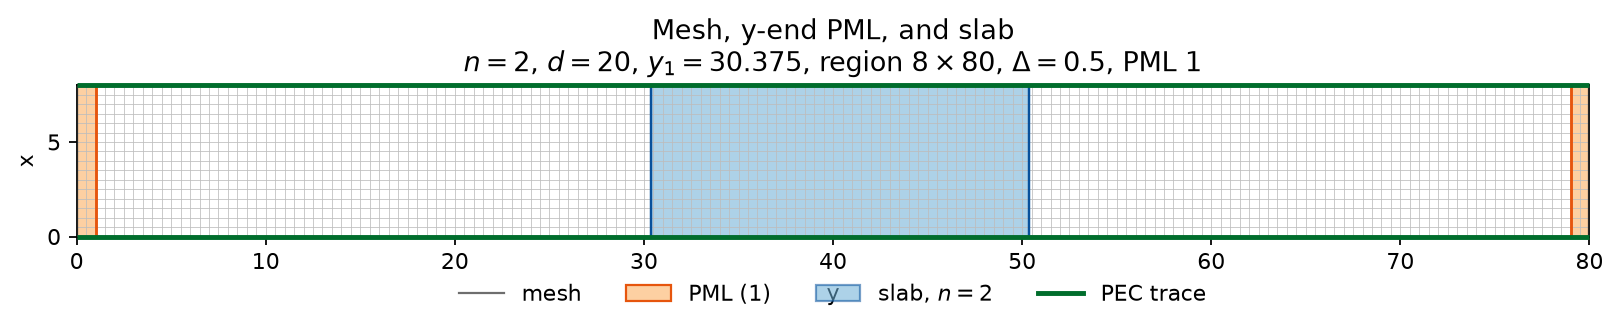
\includegraphics[width=\textwidth]{../examples/fdfd/2d/fresnel_slab_index2_d20_lam46_y130.375_length8_height80_dx0.5_pml1/domain.png}
\caption{Default Fresnel domain. Orange bands are the $y$-end PML thickness
drawn on the figure. Green edges are the PEC trace at $x=0$ and $x=8$.}
\label{fig:fresnel-domain}
\end{figure}

\begin{figure}[ht]
\centering
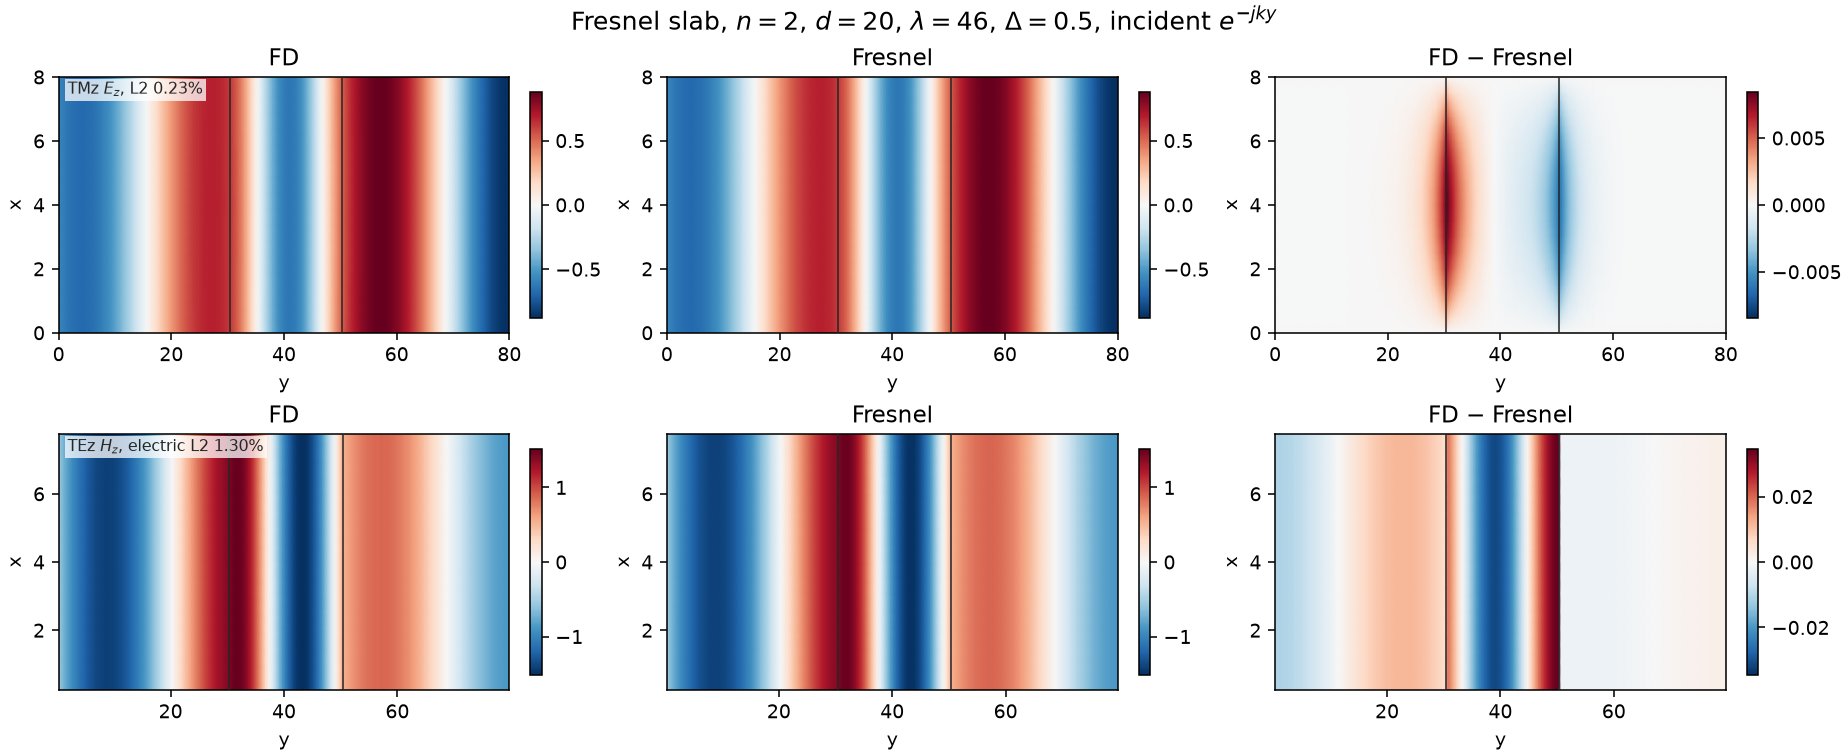
\includegraphics[width=\textwidth]{../examples/fdfd/2d/fresnel_slab_index2_d20_lam46_y130.375_length8_height80_dx0.5_pml1/fresnel_slab.png}
\caption{Default Fresnel maps. Vertical lines mark the slab faces. $H_z$ is
rebuilt with \eqref{eq:h-from-e}. The annotated $L^2$ errors are the free
electric samples.}
\label{fig:fresnel-fields}
\end{figure}

\subsection{Dielectric cylinder}
\label{sec:ex-cylinder}

\begin{verbatim}
python examples/fdfd/2d/dielectric_cylinder.py \
    --radius 10 --index 1.5 --size 50 --dx 1 --pml 8
\end{verbatim}

The region is a square of side \texttt{--size}. \texttt{--index} is again
$n$, with $\varepsilon_r=n^2$. The default $n=1.5$ is $\varepsilon_r=2.25$.
The size parameter $ka$ is held at $1$, so $k=1/a$ and the wavelength scales
with the radius. The radius must be positive and smaller than half the
side length minus the PML thickness. The default run writes
\begin{center}
\path{dielectric_cylinder_index1.5_ka1_a10_size50_dx1_pml8/}
\end{center}
with \texttt{domain.png} and \texttt{dielectric\_cylinder.png}.

The cylinder scatters in the plane of the grid, so the domain figure draws
the PML thickness on all four sides. As in the slab example, that frame is
a layout. The solve is still \eqref{eq:dirichlet} on the PEC wall, with the
Mie field as the trace and with the staircase disk as the only material
contrast. Every derivative in this solve is the centered difference of
Sec.~\ref{sec:curls}. TMz shows $\mathrm{Re}\,E_z$. TEz shows $\mathrm{Re}\,H_z$ from
\eqref{eq:h-from-e}, and the annotated $L^2$ error is the free-sample error
in $E_x$ and $E_y$. On the default grid those errors are $0.44\%$ and
$2.07\%$.

\begin{figure}[ht]
\centering
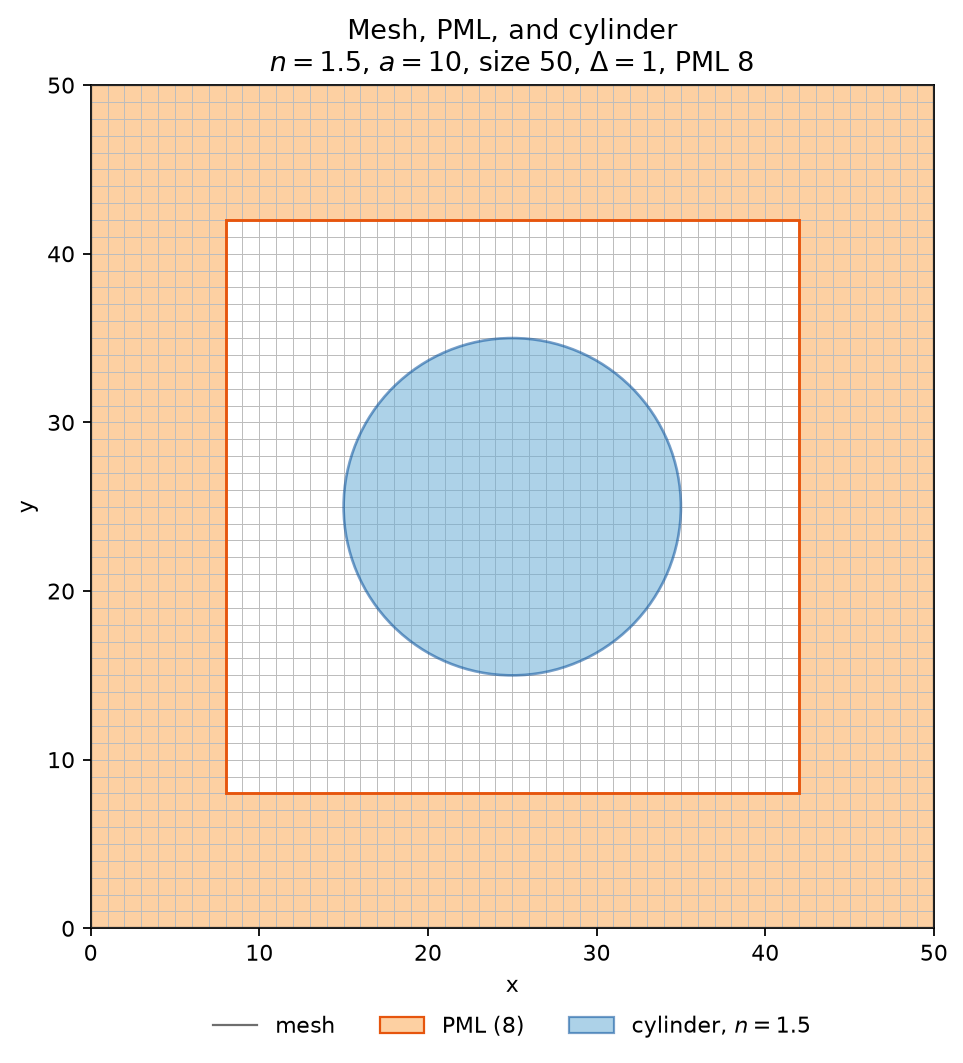
\includegraphics[width=0.72\textwidth]{../examples/fdfd/2d/dielectric_cylinder_index1.5_ka1_a10_size50_dx1_pml8/domain.png}
\caption{Default cylinder domain. The orange frame is the drawn PML
thickness. The disk is the staircase geometry. The outer boundary of the
solve remains the PEC trace.}
\label{fig:cyl-domain}
\end{figure}

\begin{figure}[ht]
\centering
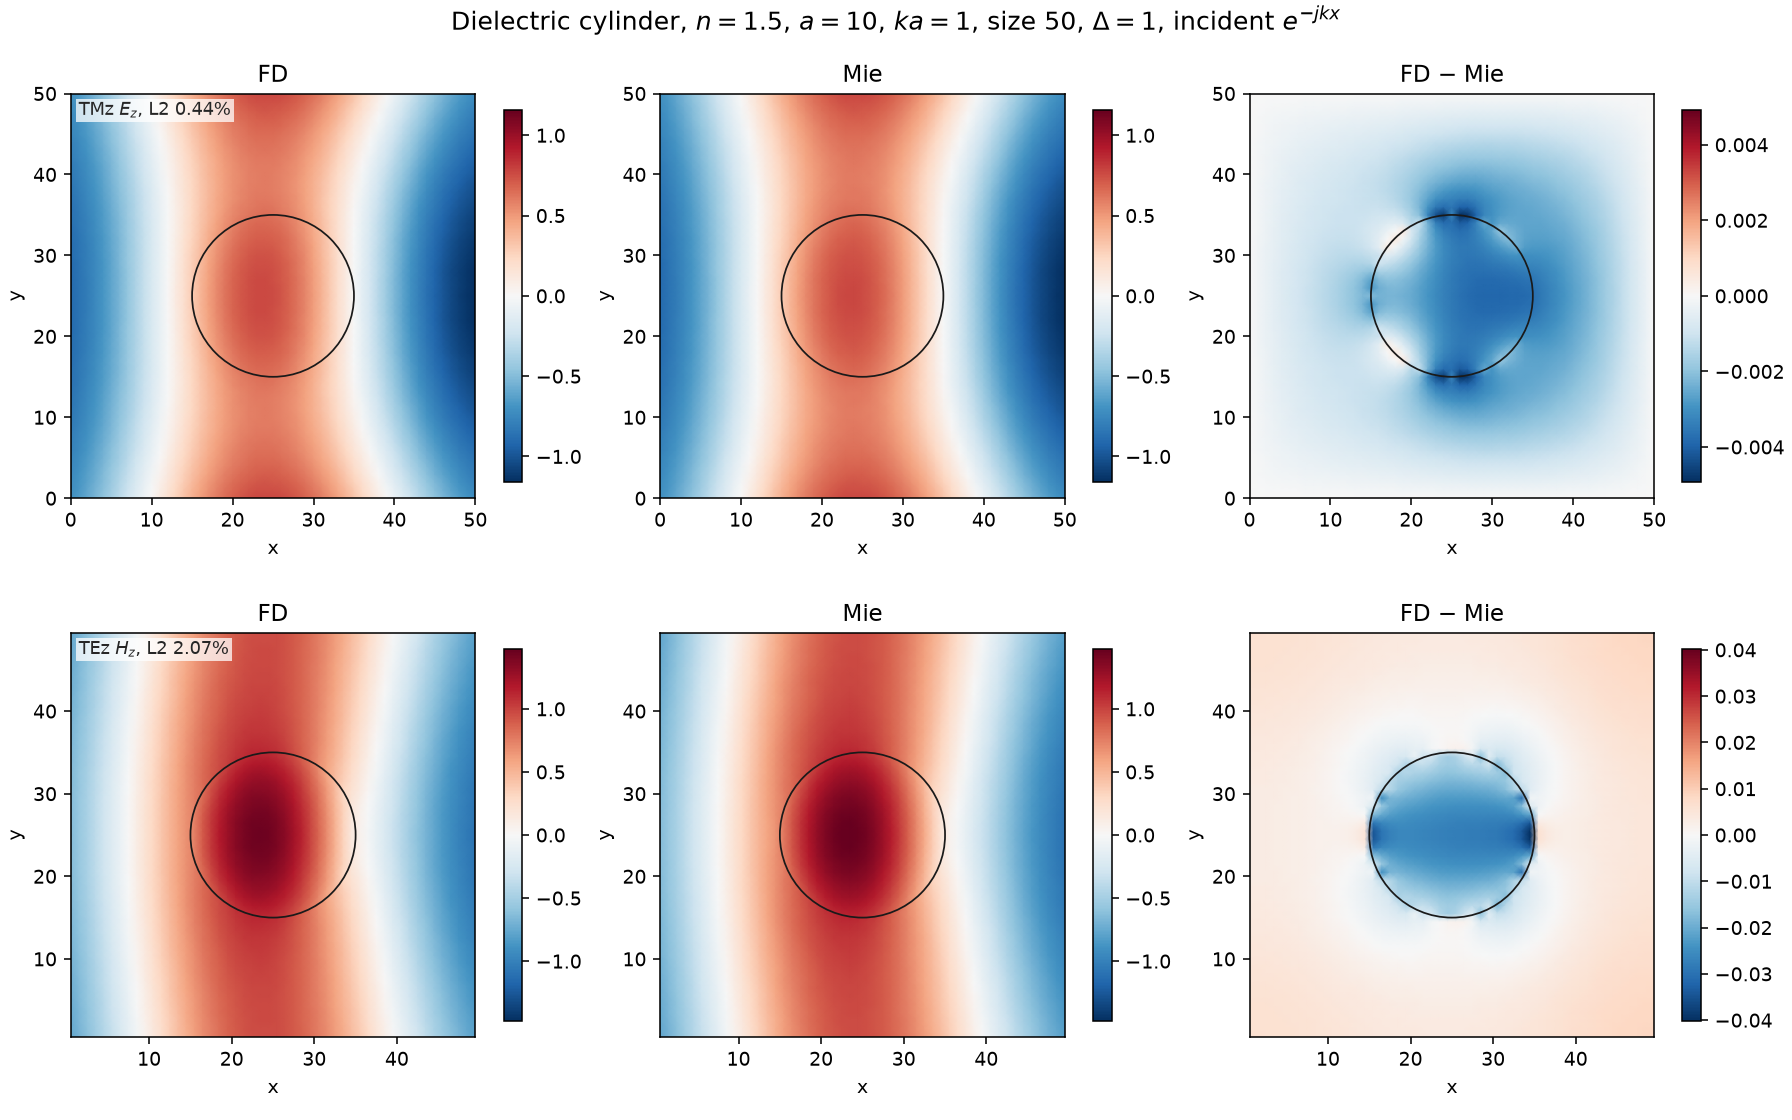
\includegraphics[width=\textwidth]{../examples/fdfd/2d/dielectric_cylinder_index1.5_ka1_a10_size50_dx1_pml8/dielectric_cylinder.png}
\caption{Default cylinder maps against the Mie series at $ka=1$, $n=1.5$.}
\label{fig:cyl-fields}
\end{figure}

\clearpage
\subsection{Line current in a PML}
\label{sec:ex-pml}

\begin{verbatim}
python examples/fdfd/2d/pml_line.py \
    --wavelength 1 --side 3 --dx 0.05 --pml 8
\end{verbatim}

The domain is a square PEC box of side \texttt{--side}. \texttt{--dx} is
the cell size, and \texttt{--side} must be an integer number of those
cells, at least two. \texttt{--pml} is the cell count on every side. It is
at least one, and twice that count stays below the number of cells, so an
interior remains. \texttt{--wavelength} is the free-space wavelength. The
source is the center $E_z$ sample, $J_z=1/(\Delta x\,\Delta y)$, and the
reference is the line current of Sec.~\ref{sec:analytics} with $I=1$. The
default run writes
\begin{center}
\path{pml_line_lam1_side3_dx0.05_pml8/}
\end{center}
and \texttt{pml\_line.png}. The orange square is the inner edge of the
band. On this grid the interior $L^2$ error, outside half a wavelength of
the source, is $2.10\%$. That number belongs to this grid. The Hankel panel
is the unbounded cylindrical wave, including through the band, so the
difference outside the square is the absorption.

\begin{figure}[ht]
\centering
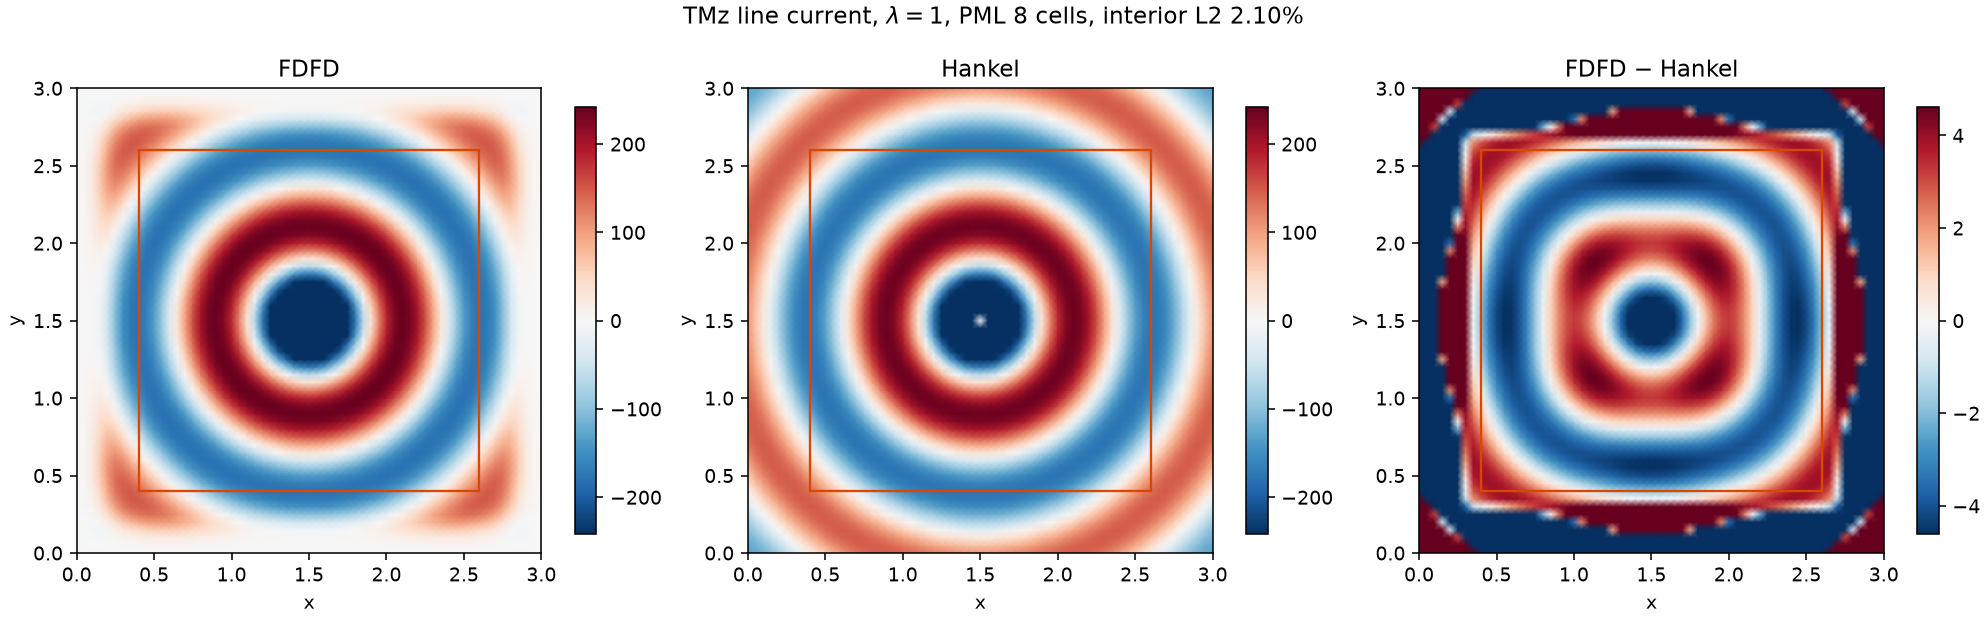
\includegraphics[width=\textwidth]{../examples/fdfd/2d/pml_line_lam1_side3_dx0.05_pml8/pml_line.png}
\caption{Line current at $\lambda=1$ on a $3\,\mathrm{m}$ box,
$\Delta=0.05\,\mathrm{m}$, with eight PML cells on each side. The orange
square is the inner edge of the band. The annotated error is the interior
window described above.}
\label{fig:pml-line}
\end{figure}

\clearpage
\subsection{Open PEC cylinder}
\label{sec:ex-pec}

\begin{verbatim}
python examples/fdfd/2d/pec_cylinder.py \
    --radius 8 --size 64 --dx 1 --pml 8
\end{verbatim}

The region is a square of side \texttt{--size}. \texttt{--pml} is the cell
count of the convolutional PML on each side, the stretch of
Sec.~\ref{sec:pml}. $ka$ stays at 1. The solve frequency is
$\omega=c_0/a$, and the Mie series uses
$k=\omega\sqrt{\mu_0\varepsilon_0}$. The radius must lie inside the
unstretched square. The default run writes
\begin{center}
\path{pec_cylinder_ka1_a8_size64_dx1_pml8/}
\end{center}
with \texttt{domain.png} and \texttt{pec\_cylinder.png}.

The unknown is the scattered field. The cylinder trace is
$-E_{\mathrm{inc}}$ and the outer wall is zero. A free sample of the total
field is $E_s+E_{\mathrm{inc}}$. TMz shows $\mathrm{Re}\,E_z$. TEz shows
$\mathrm{Re}\,H_z$ from \eqref{eq:h-from-e}. The annotated $L^2$ is the
electric-sample error on the unstretched samples at least $2\Delta$
outside the circle. On this grid those errors are $4.20\%$ (TMz) and
$5.58\%$ (TEz). The orange square is the inner edge of the PML. Outside
that square the difference is the absorption together with the scattered
field's wall condition.

\begin{figure}[ht]
\centering
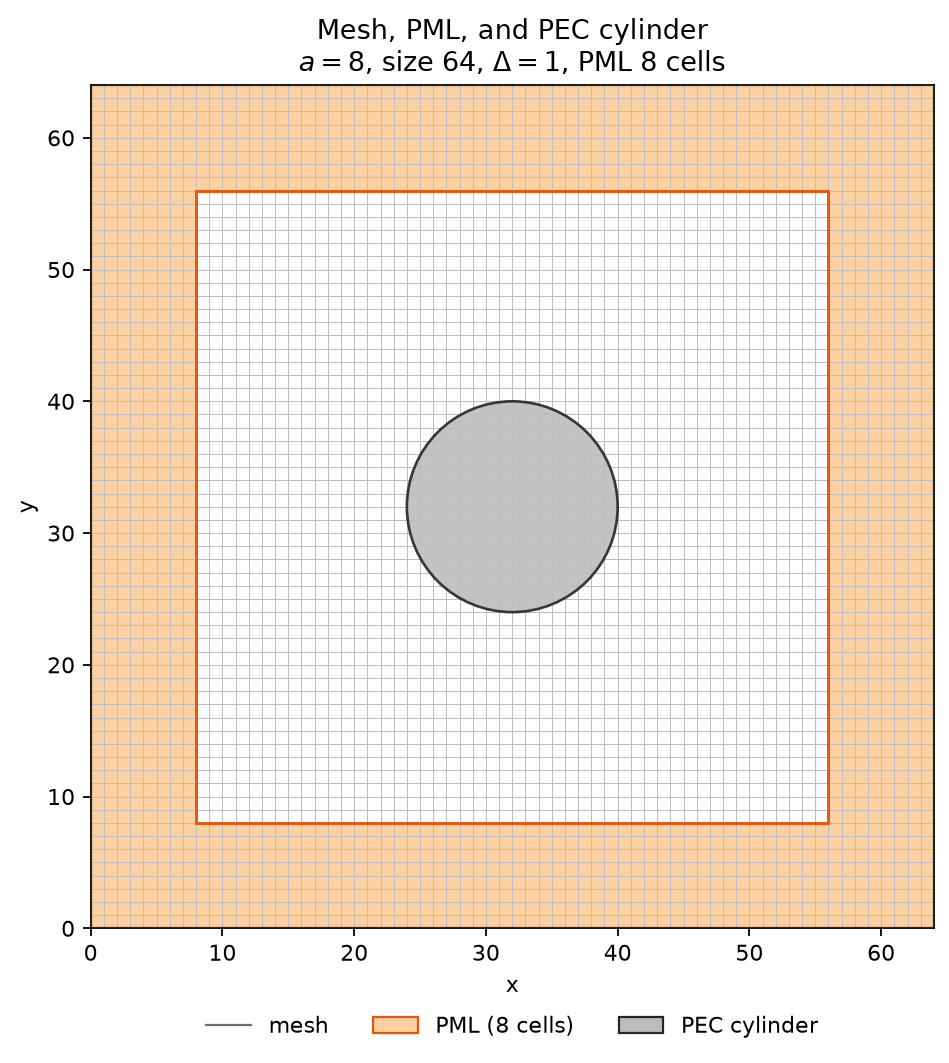
\includegraphics[width=0.72\textwidth]{../examples/fdfd/2d/pec_cylinder_ka1_a8_size64_dx1_pml8/domain.png}
\caption{Default open-cylinder domain. The orange frame is the PML band
used by the solve. The disk is the staircase PEC.}
\label{fig:pec-domain}
\end{figure}

\begin{figure}[ht]
\centering
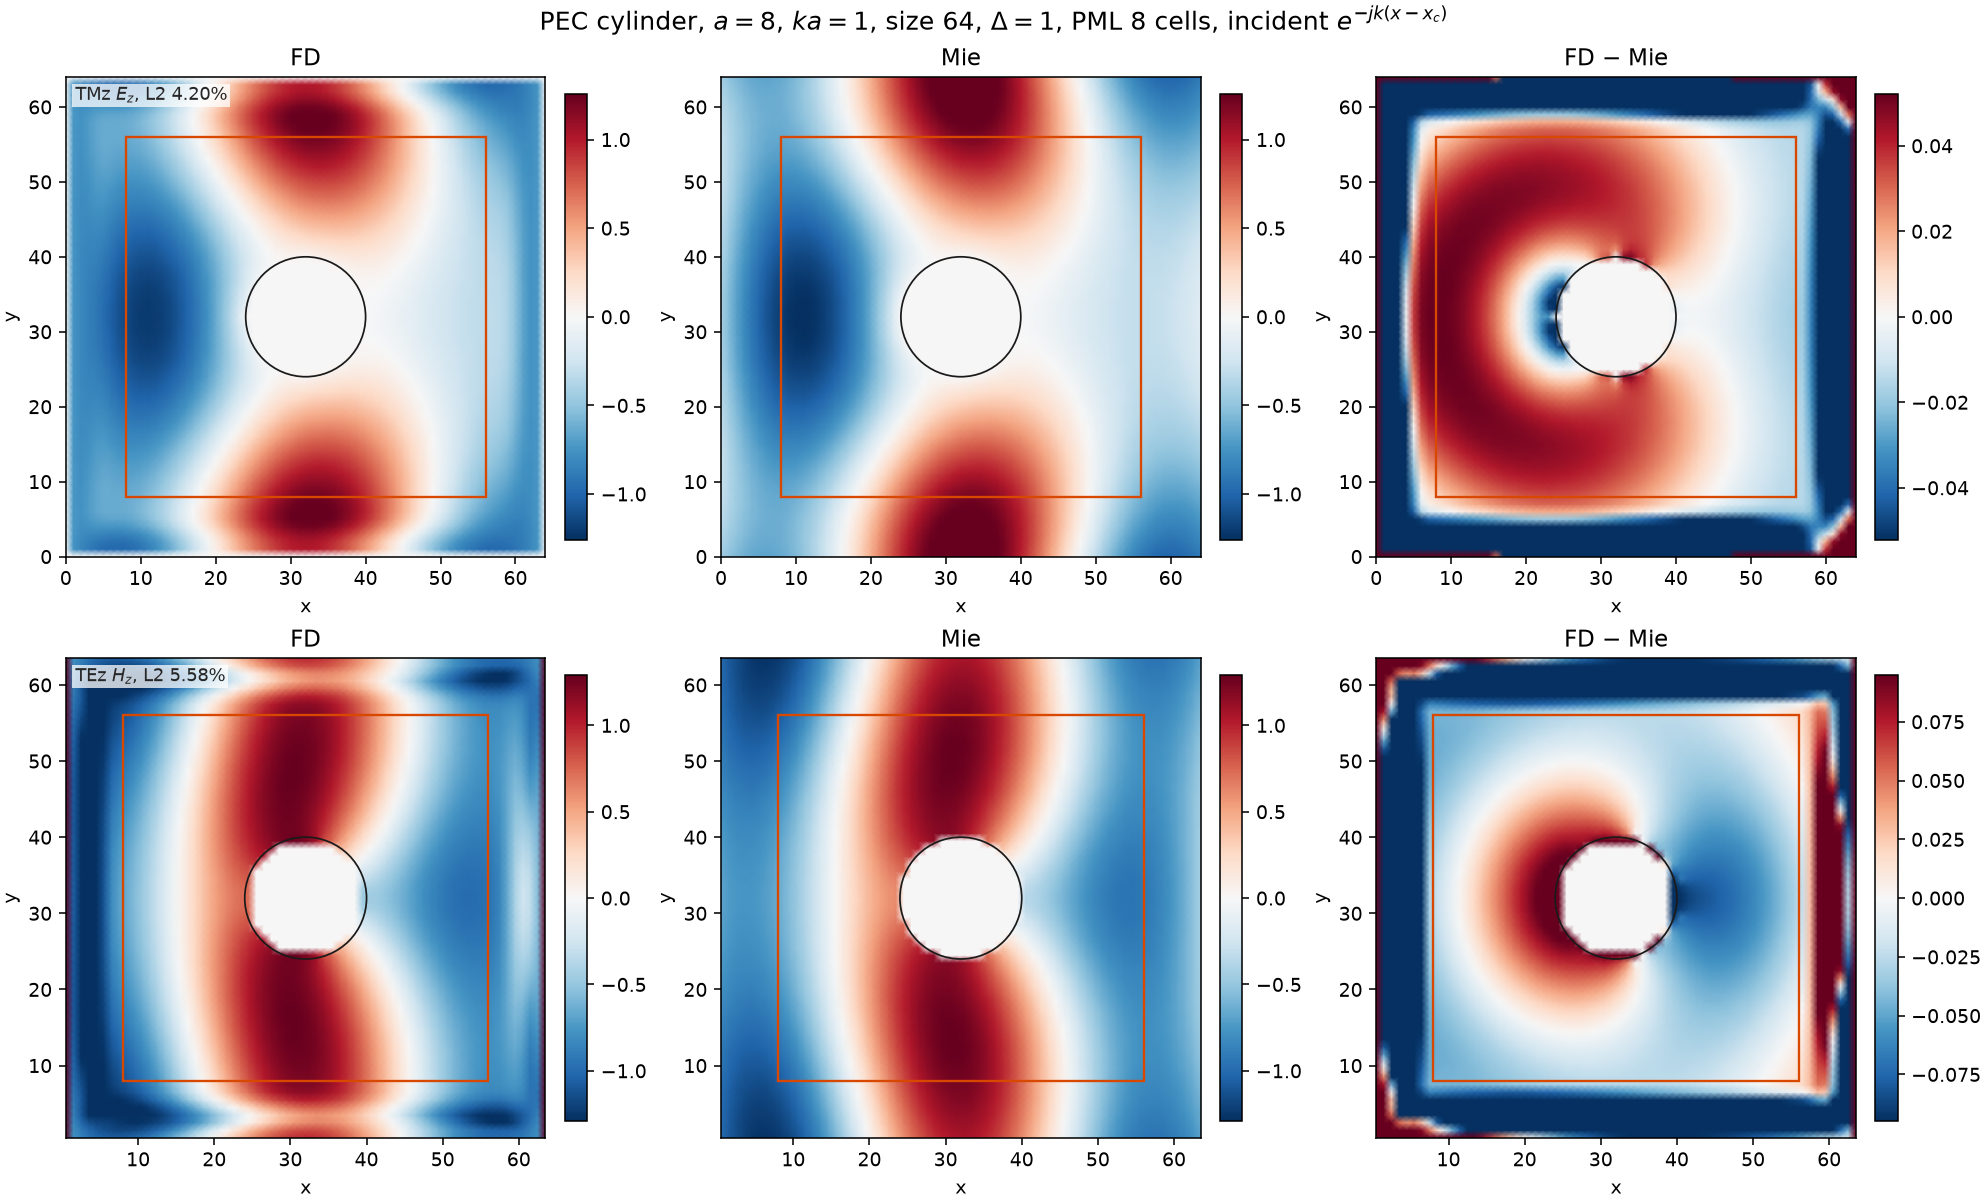
\includegraphics[width=\textwidth]{../examples/fdfd/2d/pec_cylinder_ka1_a8_size64_dx1_pml8/pec_cylinder.png}
\caption{Open PEC cylinder at $ka=1$, $a=8$, $\Delta=1$, with eight PML
cells on each side. The annotated $L^2$ errors are the electric samples
in the unstretched window, at least $2\Delta$ outside the circle.}
\label{fig:pec-fields}
\end{figure}

\clearpage
\subsection{Open dielectric cylinder}
\label{sec:ex-diel}

\begin{verbatim}
python examples/fdfd/2d/dielectric_cylinder_open.py \
    --radius 8 --index 1.5 --size 64 --dx 1 --pml 8
\end{verbatim}

The region is a square of side \texttt{--size}. \texttt{--index} is $n$,
with $\varepsilon_r=n^2$. The default $n=1.5$ is $\varepsilon_r=2.25$.
\texttt{--pml} is the cell count of the convolutional PML on each side,
the stretch of Sec.~\ref{sec:pml}. $ka$ stays at 1. The solve frequency is
$\omega=(ka/a)\,c_0$, and the Mie series uses
$k=\omega\sqrt{\mu_0\varepsilon_0}$. The radius must lie inside the
unstretched square. The default run writes
\begin{center}
\path{dielectric_cylinder_open_index1.5_ka1_a8_size64_dx1_pml8/}
\end{center}
with \texttt{domain.png} and \texttt{dielectric\_cylinder\_open.png}.

The unknown is the scattered field. The operator holds the staircase disk.
The impressed current is
$J=j\omega(\varepsilon-\varepsilon_0)E_{\mathrm{inc}}$
on the electric samples, and it is zero in the vacuum. The outer wall is a
homogeneous PEC. A free sample of the total field is
$E_s+E_{\mathrm{inc}}$. TMz shows $\mathrm{Re}\,E_z$. TEz shows
$\mathrm{Re}\,H_z$ from \eqref{eq:h-from-e}. The annotated $L^2$ is the
electric-sample error on the unstretched samples at least $2\Delta$ off
the circle, inside and outside. On this grid those errors are $0.45\%$
(TMz) and $0.71\%$ (TEz). The orange square is the inner edge of the PML.
The closed-box cylinder of Sec.~\ref{sec:ex-cylinder} still prescribes the
Mie trace and does not stretch the derivatives.

\begin{figure}[ht]
\centering
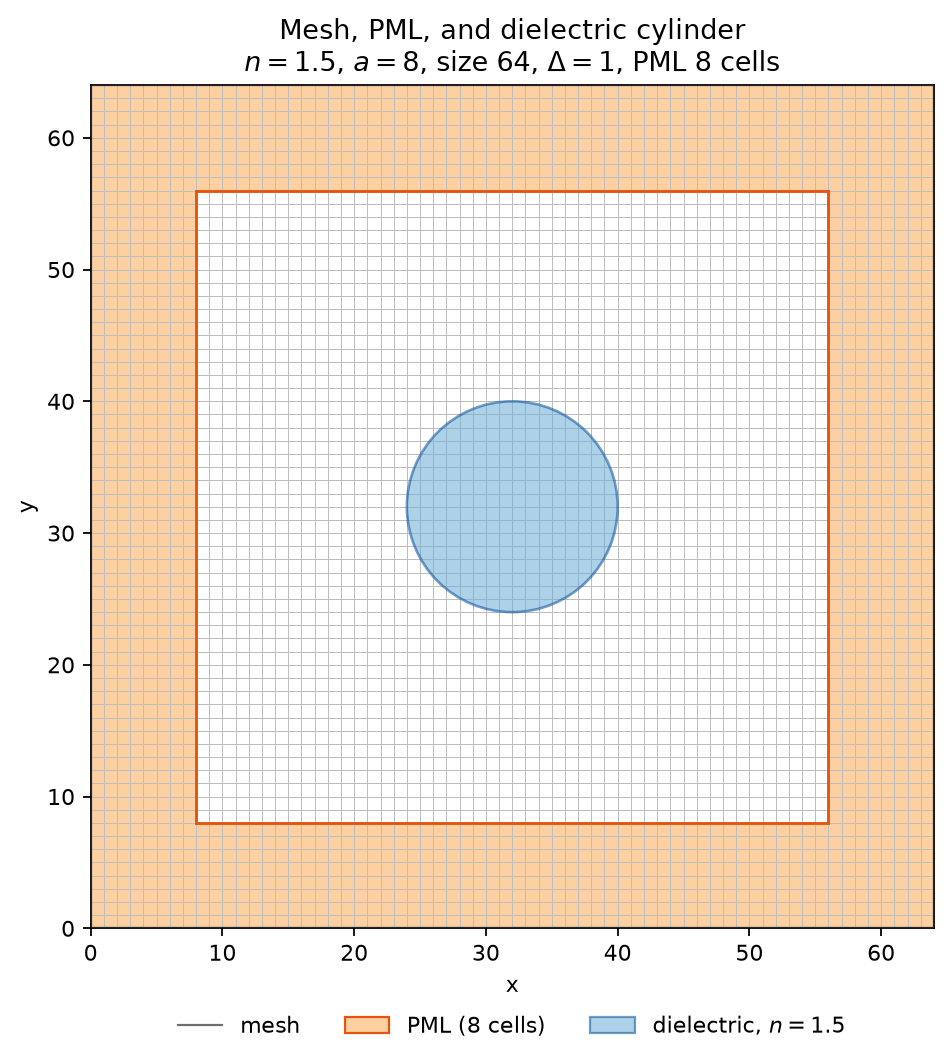
\includegraphics[width=0.72\textwidth]{../examples/fdfd/2d/dielectric_cylinder_open_index1.5_ka1_a8_size64_dx1_pml8/domain.png}
\caption{Default open dielectric domain. The orange frame is the PML band
used by the solve. The disk is the staircase dielectric, $n=1.5$.}
\label{fig:diel-open-domain}
\end{figure}

\begin{figure}[ht]
\centering
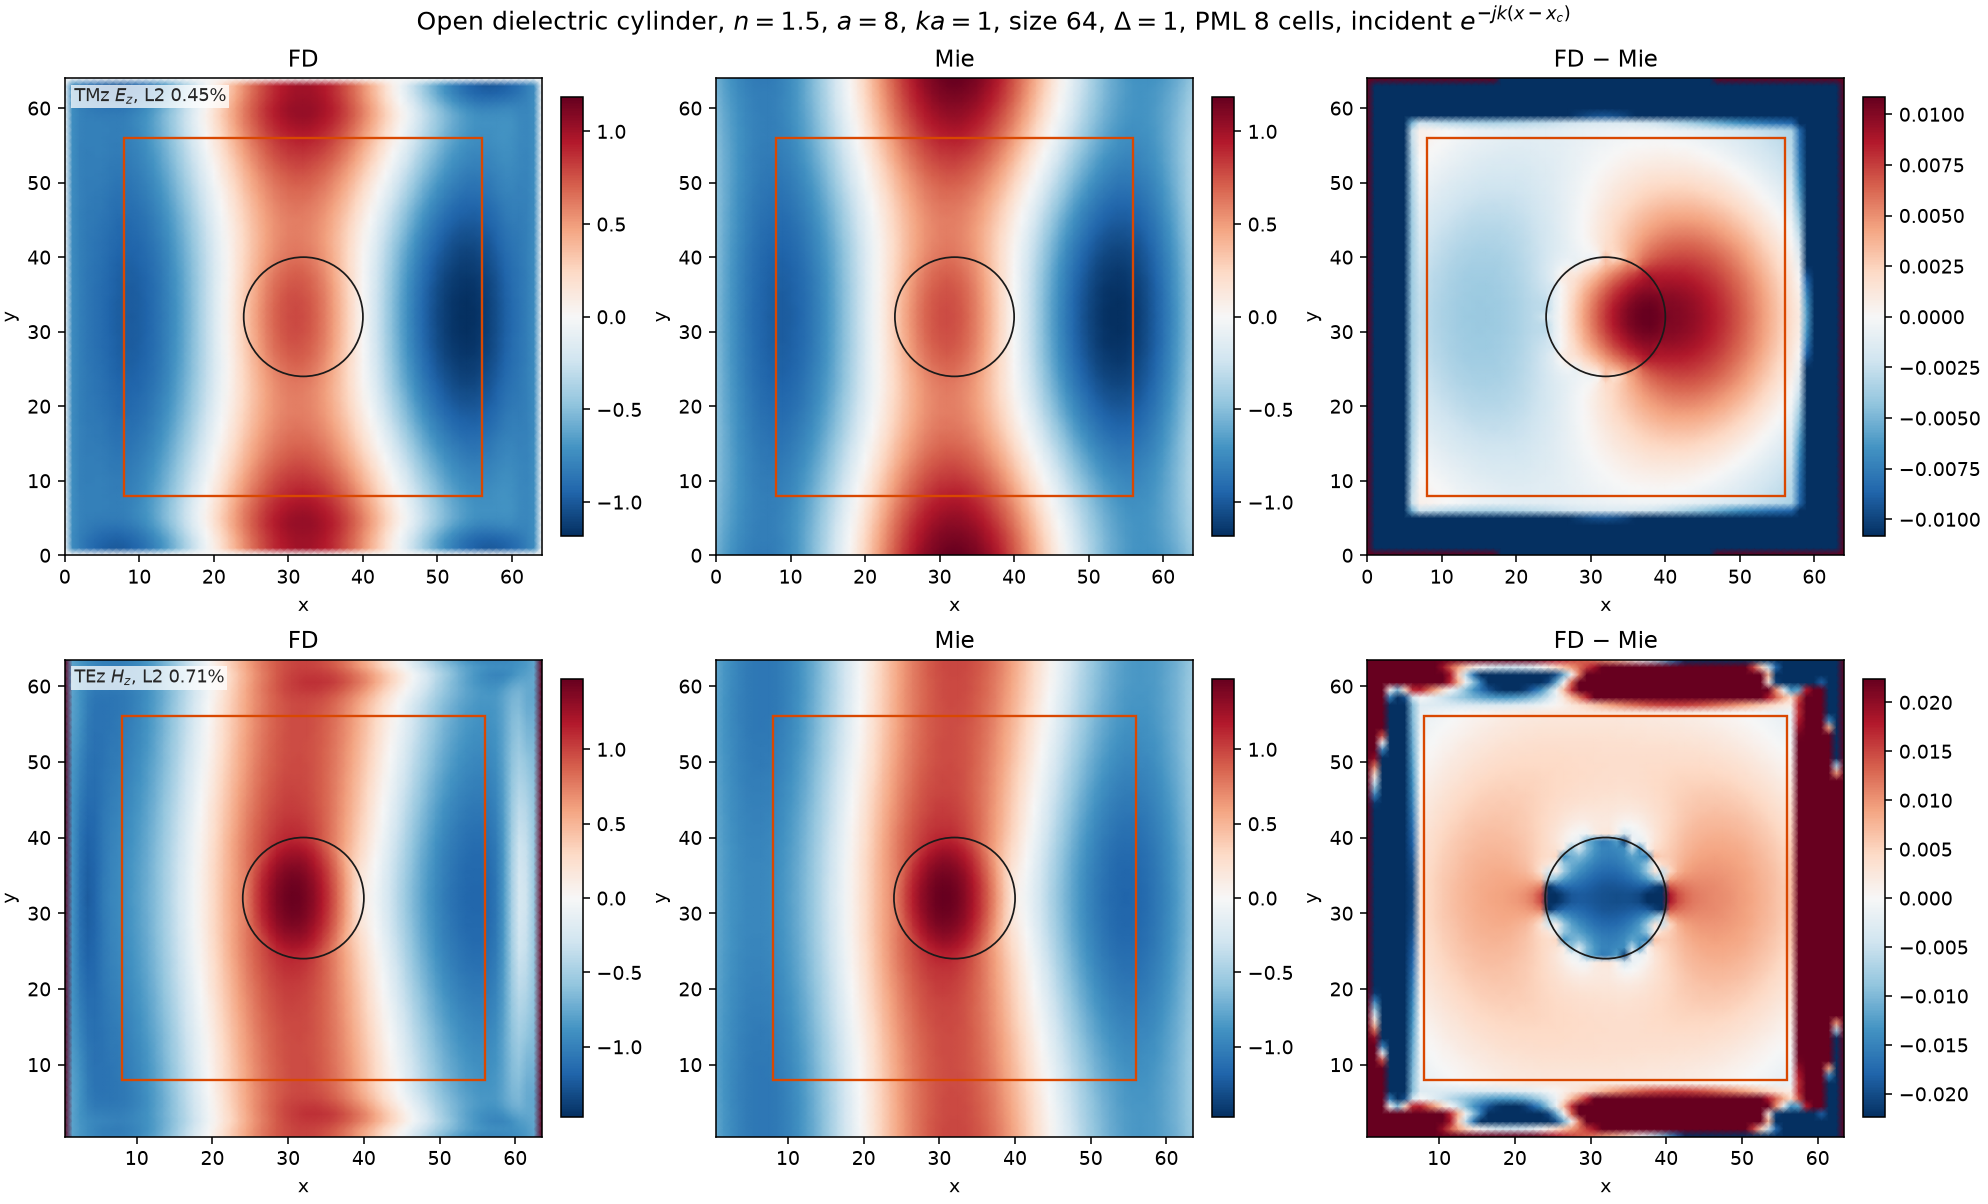
\includegraphics[width=\textwidth]{../examples/fdfd/2d/dielectric_cylinder_open_index1.5_ka1_a8_size64_dx1_pml8/dielectric_cylinder_open.png}
\caption{Open dielectric cylinder at $n=1.5$, $ka=1$, $a=8$, $\Delta=1$,
with eight PML cells on each side. The annotated $L^2$ errors are the
electric samples in the unstretched window, at least $2\Delta$ off the
circle.}
\label{fig:diel-open-fields}
\end{figure}

\subsection{3D PEC cavity}
\label{sec:ex-cavity}

\begin{verbatim}
python examples/fdfd/3d/cavity.py --nx 16 --ny 12 --nz 10 --dx 1
\end{verbatim}

The box is a PEC cavity with one spacing on every axis. The default run
writes
\begin{center}
\path{cavity_nx16_ny12_nz10_dx1/}
\end{center}
with \texttt{cavity.png}. The three panels are the pure modes $(1,1,0)$,
$(1,0,1)$, and $(0,1,1)$. Each panel shows the one nonzero electric
component, on the plane in which that mode varies. The script prints the
relative Rayleigh residual of each mode on that grid. The regression in
the test suite uses the coarser $8\times 6\times 5$ box and the bar
$10^{-10}$.

\begin{figure}[ht]
\centering
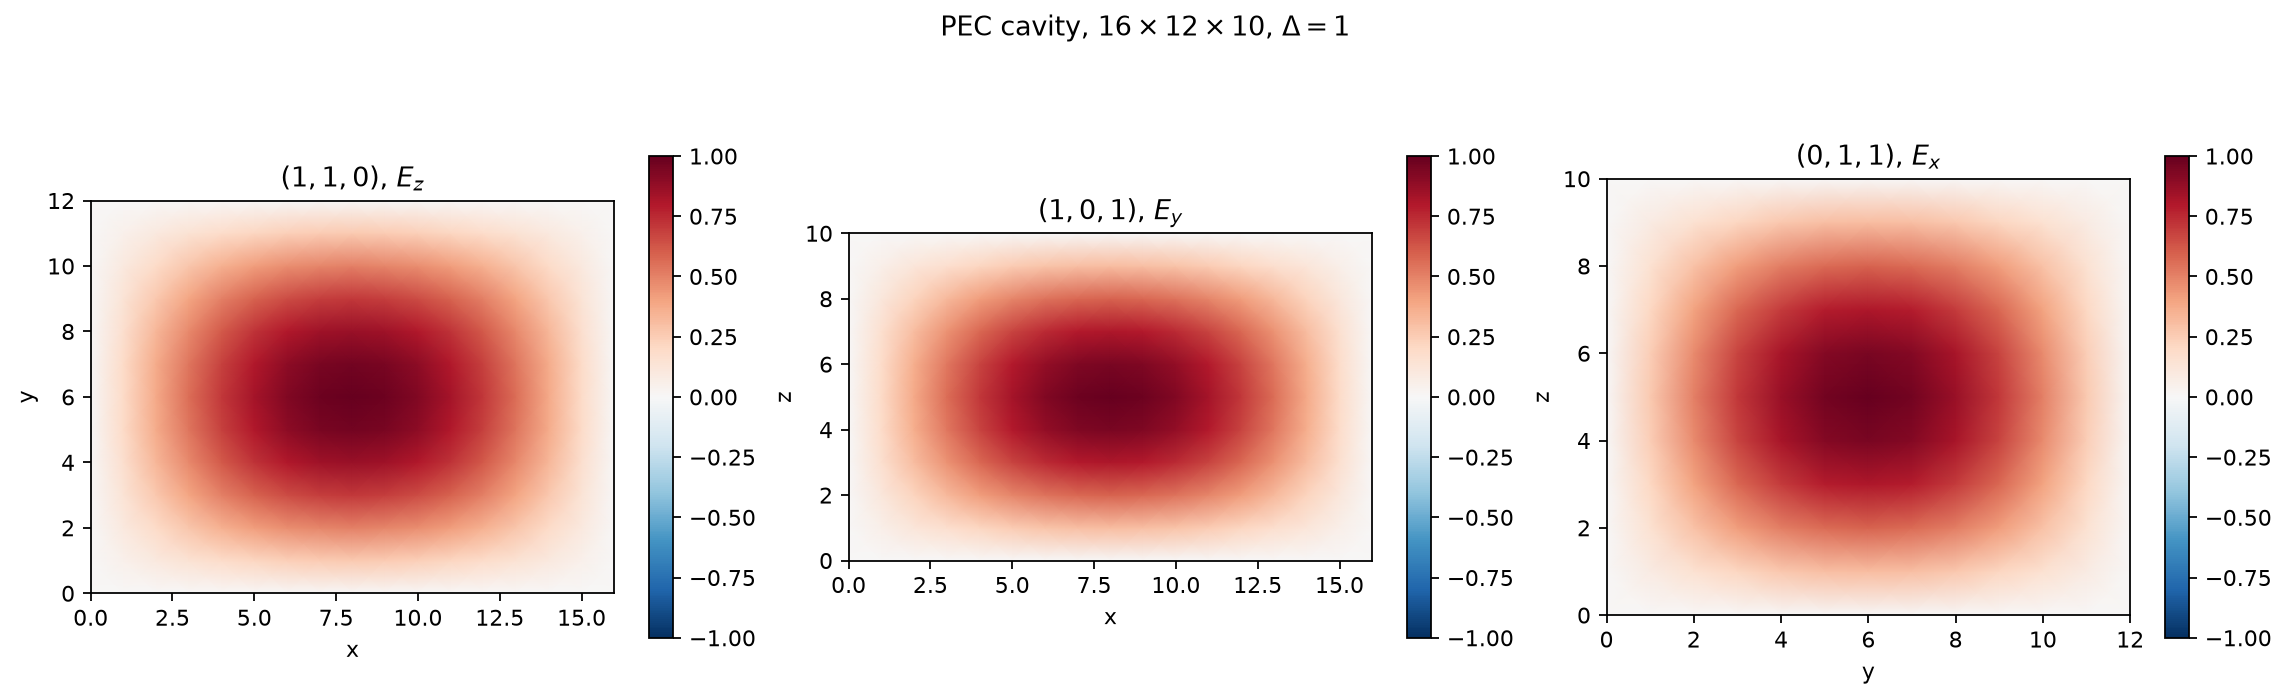
\includegraphics[width=\textwidth]{../examples/fdfd/3d/cavity_nx16_ny12_nz10_dx1/cavity.png}
\caption{Pure modes of a $16\times 12\times 10$ PEC cavity at $\Delta=1$.
$(1,1,0)$ is $E_z(x,y)$, $(1,0,1)$ is $E_y(x,z)$, and $(0,1,1)$ is
$E_x(y,z)$.}
\label{fig:cavity3d}
\end{figure}

\subsection{Open dielectric sphere}
\label{sec:ex-sphere}

\begin{verbatim}
python examples/fdfd/3d/dielectric_sphere.py \
    --radius 4 --index 1.5 --size 18 --dx 1 --pml 3
\end{verbatim}

The default run writes
\begin{center}
\path{dielectric_sphere_index1.5_ka1_a4_size18_dx1_pml3/}
\end{center}
with \texttt{domain.png} and \texttt{dielectric\_sphere.png}. The cube is
$18$ cells on a side at $\Delta=1$, the radius is $4$, the index is $1.5$,
and $ka=1$. Three PML cells back every face. The unknown is the scattered
field. The staircase ball stays in the operator, and the incident wave
$\hat{\mathbf{x}}\,e^{-jk(z-z_c)}$ enters as the contrast current. The
figure shows $\mathrm{Re}\,E_x$ on the $xz$ plane through the center. The
annotated $L^2$ is the electric-sample error on all three components,
outside the PML and at least $2\Delta$ off the surface. On this grid that
error is $0.98\%$. The regression uses the same grid and the bar
$1.8\times 10^{-2}$.

\begin{figure}[ht]
\centering
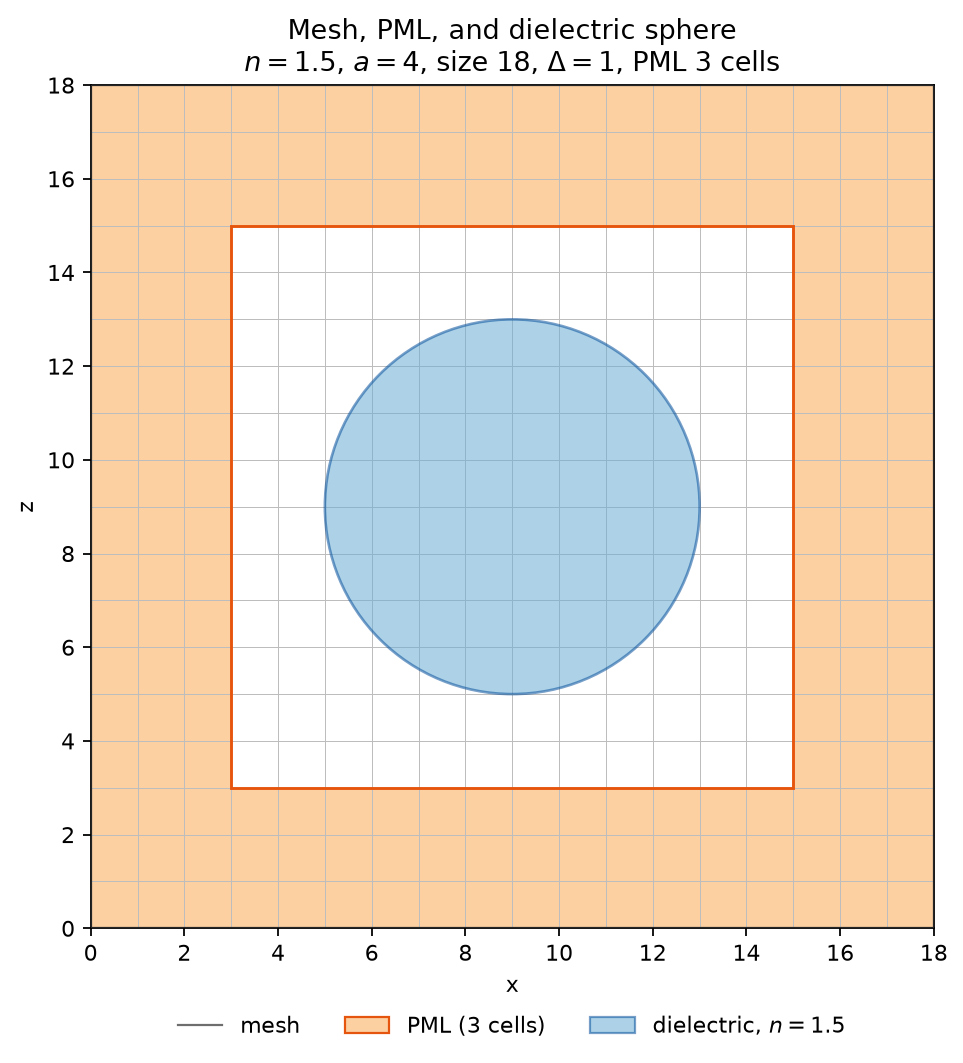
\includegraphics[width=0.72\textwidth]{../examples/fdfd/3d/dielectric_sphere_index1.5_ka1_a4_size18_dx1_pml3/domain.png}
\caption{Default open-sphere domain. The orange frame is the PML band
used by the solve. The disk is the cross-section of the staircase ball,
$n=1.5$.}
\label{fig:sphere-domain}
\end{figure}

\begin{figure}[ht]
\centering
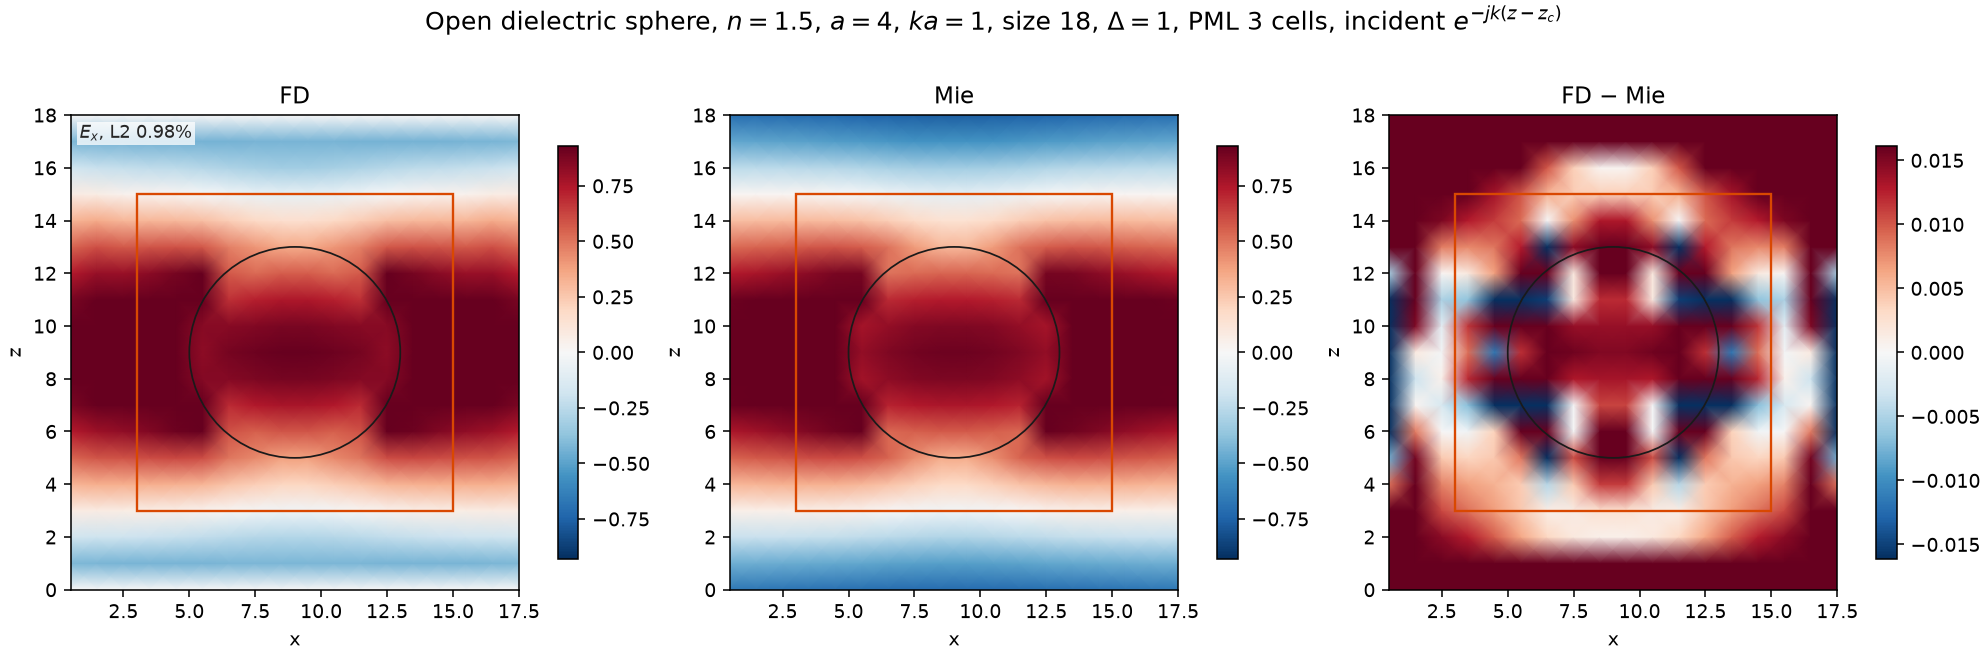
\includegraphics[width=\textwidth]{../examples/fdfd/3d/dielectric_sphere_index1.5_ka1_a4_size18_dx1_pml3/dielectric_sphere.png}
\caption{Open dielectric sphere at $n=1.5$, $ka=1$, $a=4$, on an $18^3$
box at $\Delta=1$, with three PML cells on each face. The panels are
$\mathrm{Re}\,E_x$ on the $xz$ plane through the center. The annotated
$L^2$ is the electric-sample error outside the PML and at least $2\Delta$
off the surface.}
\label{fig:sphere-fields}
\end{figure}

\clearpage
\subsection{Hertzian dipole}
\label{sec:ex-dipole}

\begin{verbatim}
python examples/fdfd/3d/hertzian_dipole.py
\end{verbatim}

The element is $z$-directed with moment $I\ell=1$. It sits on the $E_z$
sample nearest the center of a PEC cube, and that sample carries
$J_z=1/(\Delta x\Delta y\Delta z)$. \texttt{--wavelength}, \texttt{--size},
\texttt{--dx}, and \texttt{--pml} are the free-space wavelength, the cube
side, the cell size, and the PML depth on each face. The defaults are
$1$, $1.6$, $0.1$, and $3$. The comparison is every free electric sample
outside the PML and at least $0.25\lambda$ from the element.

The default run writes
\begin{center}
\path{hertzian_dipole_lam1_size1.6_dx0.1_pml3/}
\end{center}
with \texttt{domain.png} and \texttt{hertzian\_dipole.png}. The cube is
$16$ cells on a side. Three PML cells back every face. The figure shows
$\mathrm{Re}\,E_z$ on the $xz$ plane through the element. On this grid
the annotated $L^2$ is $9.65\%$. The regression uses the same grid and
the bar $0.16$.

\begin{figure}[ht]
\centering
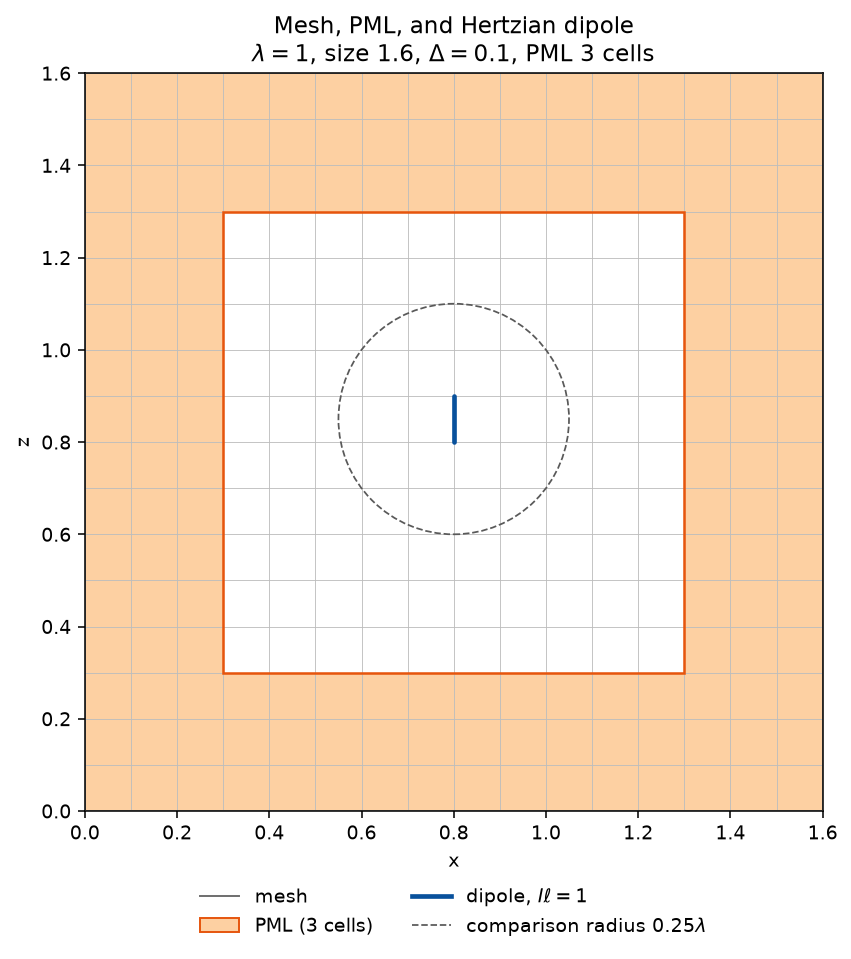
\includegraphics[width=0.72\textwidth]{../examples/fdfd/3d/hertzian_dipole_lam1_size1.6_dx0.1_pml3/domain.png}
\caption{Default Hertzian-dipole domain. The orange frame is the PML
band used by the solve. The blue segment is the $z$-directed element.
The dashed circle is the $0.25\lambda$ radius inside which the field
comparison is omitted.}
\label{fig:dipole-domain}
\end{figure}

\begin{figure}[ht]
\centering
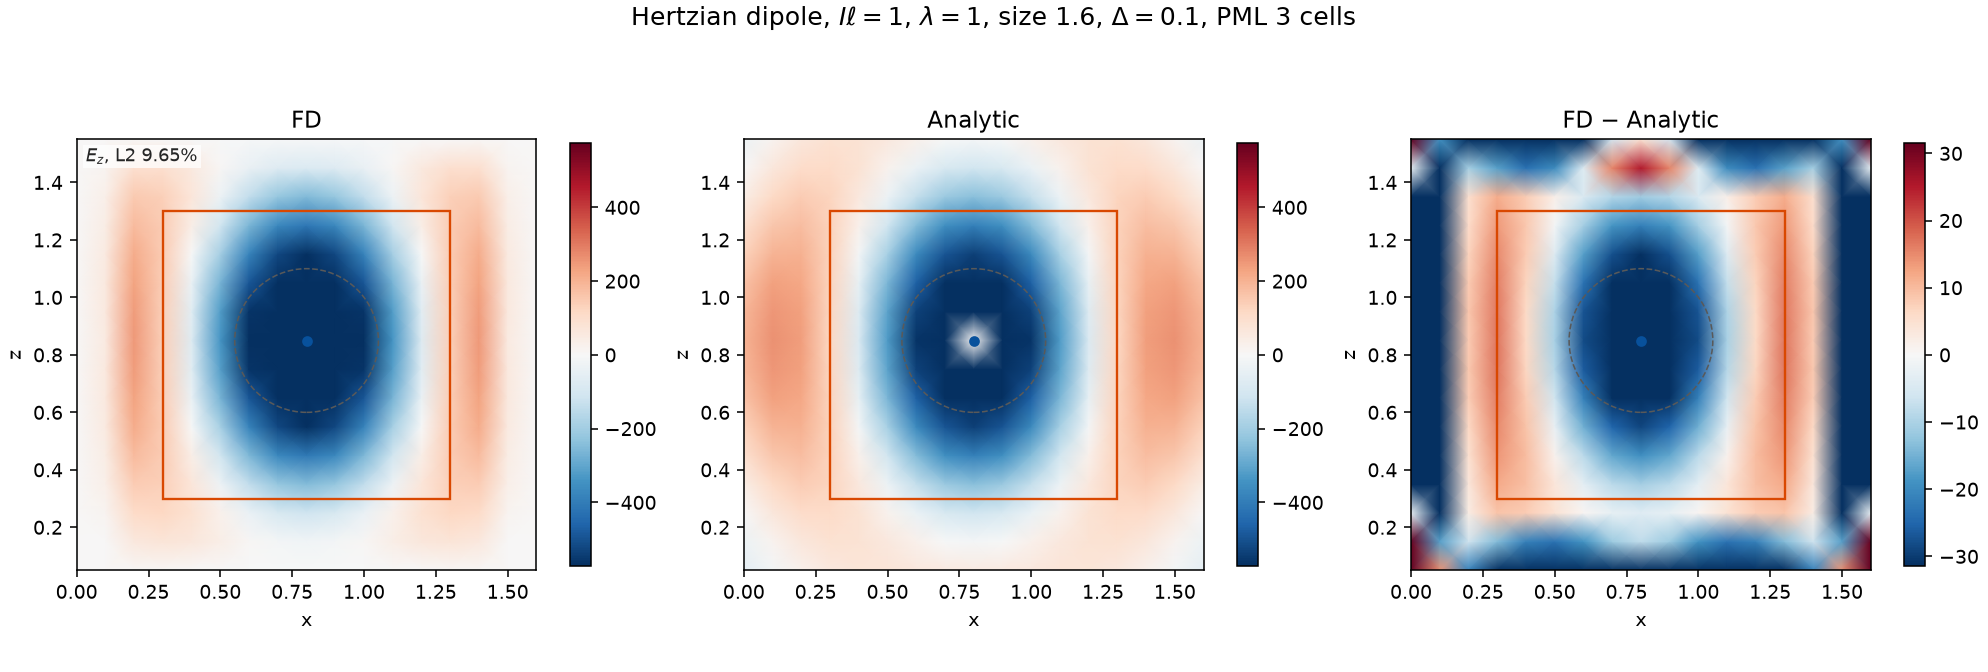
\includegraphics[width=\textwidth]{../examples/fdfd/3d/hertzian_dipole_lam1_size1.6_dx0.1_pml3/hertzian_dipole.png}
\caption{Hertzian dipole of moment $I\ell=1$ at $\lambda=1$, on a cube
of side $1.6$ at $\Delta=0.1$, with three PML cells on each face. The
panels are $\mathrm{Re}\,E_z$ on the $xz$ plane through the element.
The annotated $L^2$ is the electric-sample error outside the PML and at
least $0.25\lambda$ from the element.}
\label{fig:dipole-fields}
\end{figure}

\clearpage
\subsection{Resistive sheet}
\label{sec:ex-sheet}

\begin{verbatim}
python examples/fdfd/2d/resistive_sheet.py
\end{verbatim}

\texttt{--zs} is the surface impedance in ohms per square. The default is
$\eta_0$. \texttt{--wavelength}, \texttt{--y}, \texttt{--length},
\texttt{--height}, and \texttt{--dx} are the free-space wavelength, the
sheet coordinate, the two sides, and the cell size. Both sides must be a
positive integer number of cells, and the sheet must lie in
$(0,\texttt{height})$.

The default run writes
\begin{center}
\path{resistive_sheet_zs376.730313462_lam46_y40_length8_height80_dx1/}
\end{center}
with \texttt{domain.png} and \texttt{resistive\_sheet.png}. The box is
$8\times 80$ cells at $\Delta=1$. The sheet sits at $y=40$, on an electric
node, with $Z_s=\eta_0$ and $\lambda=46$. The impressed current is zero.
The wall carries the analytic trace. TMz prescribes $E_z(y)$ and TEz
prescribes $E_x(y)$ with $E_y=0$. Figure~\ref{fig:sheet-cell} is the
Ampere cell used for this run: the sheet lies on electric row $j$. The
field figure shows $\mathrm{Re}\,E_z$ and
$\mathrm{Re}\,E_x$, with propagation along the horizontal axis. On this
grid the annotated errors are $0.02\%$ (TMz) and $0.42\%$ (TEz). The
regression uses the same grid and the bars $6\times 10^{-4}$ and
$1.2\times 10^{-2}$.

\begin{figure}[ht]
\centering
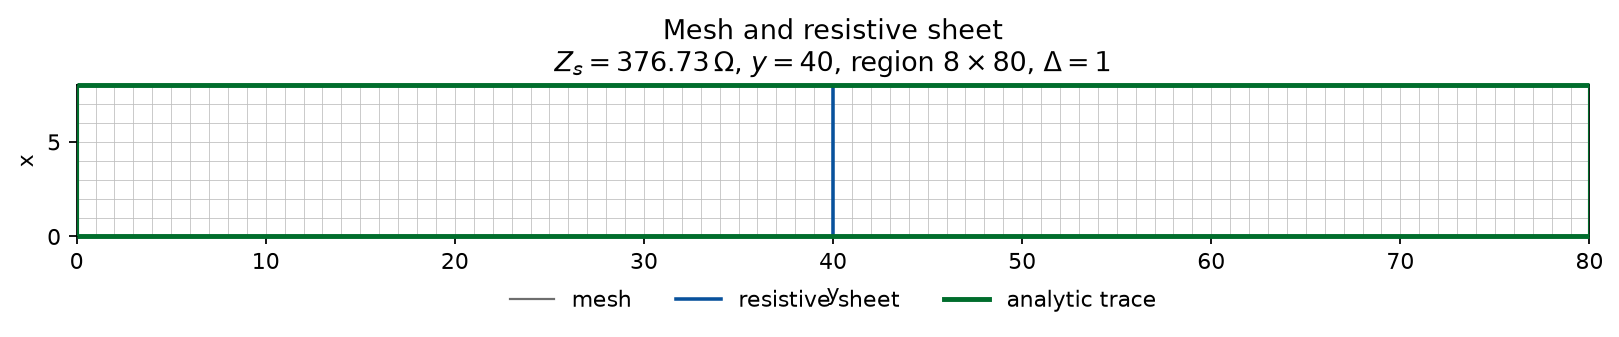
\includegraphics[width=\textwidth]{../examples/fdfd/2d/resistive_sheet_zs376.730313462_lam46_y40_length8_height80_dx1/domain.png}
\caption{Default resistive-sheet domain. The blue line is the sheet. The
green frame is the analytic trace on all four walls.}
\label{fig:sheet-domain}
\end{figure}

\begin{figure}[ht]
\centering
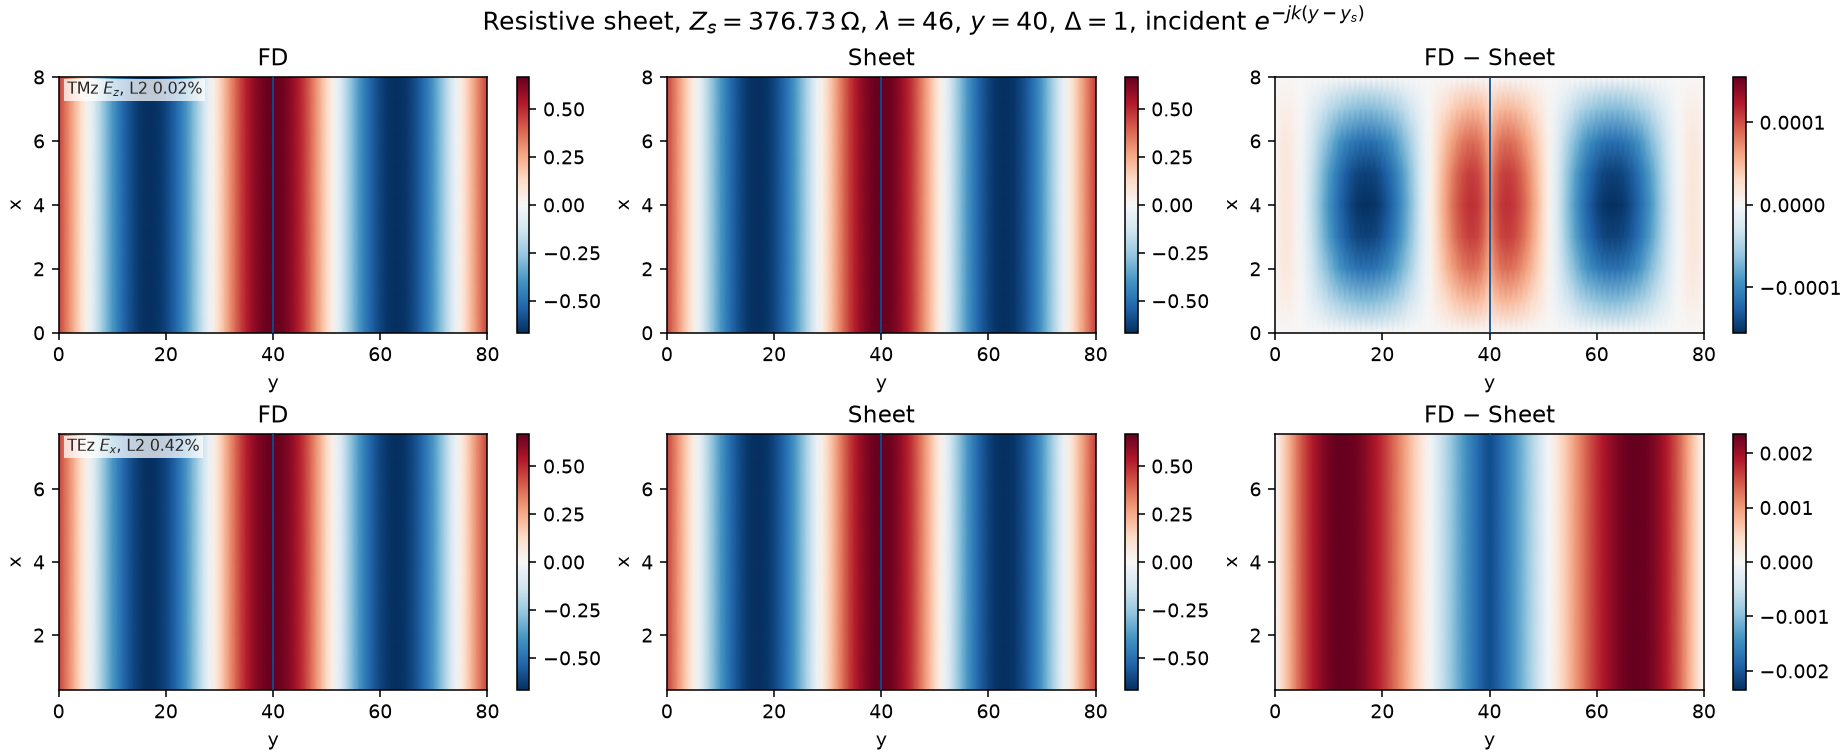
\includegraphics[width=\textwidth]{../examples/fdfd/2d/resistive_sheet_zs376.730313462_lam46_y40_length8_height80_dx1/resistive_sheet.png}
\caption{Resistive sheet at $Z_s=\eta_0$, $\lambda=46$, $y=40$, on an
$8\times 80$ box at $\Delta=1$. The rows are $\mathrm{Re}\,E_z$ (TMz) and
$\mathrm{Re}\,E_x$ (TEz). The annotated $L^2$ is the packed free electric
vector.}
\label{fig:sheet-fields}
\end{figure}

\subsection{Symmetric sheet}
\label{sec:ex-gstc}

\begin{verbatim}
python examples/fdfd/2d/symmetric_sheet.py
\end{verbatim}

\texttt{--chi-ee} and \texttt{--chi-mm} are the tangential susceptibilities.
The defaults are $0.5$ and $0.25$. \texttt{--wavelength}, \texttt{--y},
\texttt{--length}, \texttt{--height}, and \texttt{--dx} are the free-space
wavelength, the magnetic-face coordinate, the two sides, and the cell size.
Both sides must be a positive integer number of cells, and the sheet must
lie on one magnetic face inside $(0,\texttt{height})$.

The default run writes
\begin{center}
\path{symmetric_sheet_chiee0.5_chimm0.25_lam46_y40.5_length8_height80_dx1/}
\end{center}
with \texttt{domain.png} and \texttt{symmetric\_sheet.png}. The box is
$8\times 80$ cells at $\Delta=1$. The sheet sits at $y=40.5$, halfway
between electric rows, with $\chi_{ee}=0.5$, $\chi_{mm}=0.25$, and
$\lambda=46$. Figure~\ref{fig:gstc-cell} is that face. The impressed current is zero. The wall carries the analytic
trace. TMz prescribes $E_z(y)$ and TEz prescribes $E_x(y)$ with $E_y=0$.
The field figure shows $\mathrm{Re}\,E_z$ and $\mathrm{Re}\,E_x$, with
propagation along the horizontal axis. On this grid the annotated errors
are $1.39\%$ (TMz) and $6.39\%$ (TEz). The regression uses the same grid
and the bars $4.2\times 10^{-2}$ and $1.9\times 10^{-1}$. A cell of
$\Delta=1/3$ on the same sheet drops both errors by more than half.

\begin{figure}[ht]
\centering
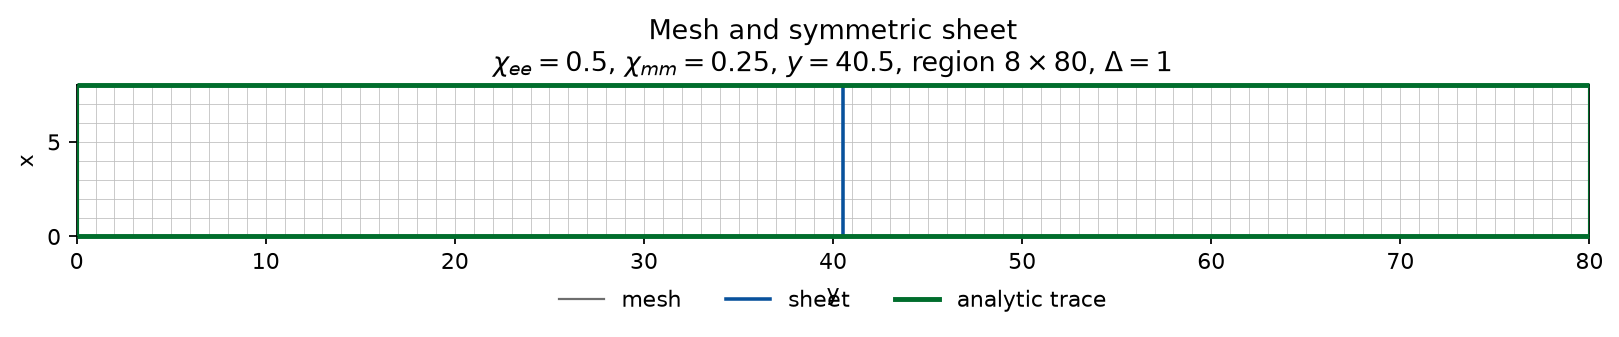
\includegraphics[width=\textwidth]{../examples/fdfd/2d/symmetric_sheet_chiee0.5_chimm0.25_lam46_y40.5_length8_height80_dx1/domain.png}
\caption{Default symmetric-sheet domain. The blue line is the sheet on a
magnetic face. The green frame is the analytic trace on all four walls.}
\label{fig:gstc-domain}
\end{figure}

\begin{figure}[ht]
\centering
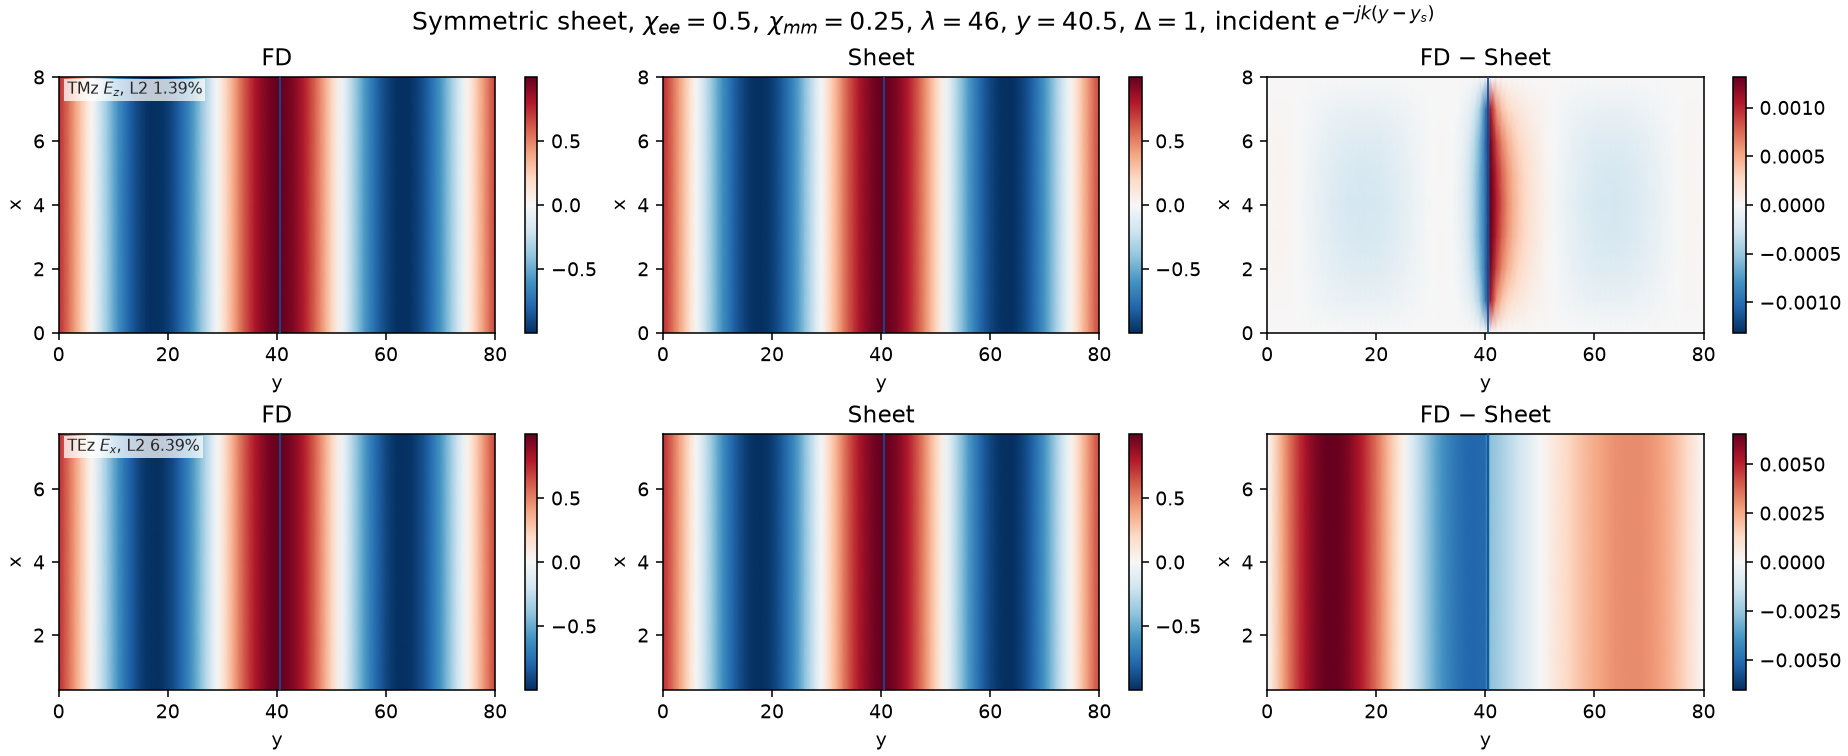
\includegraphics[width=\textwidth]{../examples/fdfd/2d/symmetric_sheet_chiee0.5_chimm0.25_lam46_y40.5_length8_height80_dx1/symmetric_sheet.png}
\caption{Symmetric sheet at $\chi_{ee}=0.5$, $\chi_{mm}=0.25$, $\lambda=46$,
$y=40.5$, on an $8\times 80$ box at $\Delta=1$. The rows are
$\mathrm{Re}\,E_z$ (TMz) and $\mathrm{Re}\,E_x$ (TEz). The annotated $L^2$
is the packed free electric vector.}
\label{fig:gstc-fields}
\end{figure}

\subsection{Finite absorbing sheet}
\label{sec:ex-finite}

\begin{verbatim}
python examples/fdfd/2d/finite_sheet.py
\end{verbatim}

\texttt{--sheet} is the sheet length in wavelengths. The default is $10$.
\texttt{--theta} is the incidence angle in degrees, measured from the sheet
normal, and the default is $0$. \texttt{--wavelength}, \texttt{--points},
and \texttt{--pml} are the free-space wavelength, the cells per wavelength,
and the PML depth on each side. The susceptibilities are
$\chi_{ee}=\chi_{mm}=-2j/k$, so a uniform sheet of this normal has
$R=T=0$ at $\theta=0$. Passing \texttt{--chi-ee}, \texttt{--chi-mm}, and
\texttt{--chi-nn} together replaces that absorber.
\texttt{--chi-em} and \texttt{--chi-me} default to zero. The absorber
rejects a nonzero value. Section~\ref{sec:ex-finite-cross} sets them
with the three real susceptibilities.
Section~\ref{sec:ex-finite-oblique} is that run at $30^\circ$. The domain leaves two wavelengths of vacuum
between the sheet and the PML. The sheet lies on the magnetic face half a
cell below mid-height. The local jump is the normal-incidence cell of
Figure~\ref{fig:gstc-cell}. The angle enters only through the incident phase
$e^{-jk(\sin\theta\,(x-x_c)+\cos\theta\,(y-y_s))}$, with phase zero at the
sheet center.

The default run writes
\begin{center}
\path{finite_sheet_lam1_points20_theta0_pml12_sheet10/}
\end{center}
with \texttt{domain.png} and \texttt{finite\_sheet.png}. The sheet is
$10\lambda$ long at $20$ cells per wavelength, with $12$ PML cells on each
side and $\theta=0$. The unknown is the scattered field. The incident
electric amplitude is $1$. The field figure shows $\mathrm{Re}\,E_z$ (TMz)
and $\mathrm{Re}\,E_x$ (TEz). On this grid the annotated means, over the
central $6\lambda$ of the sheet, are a lit-side $|E|$ of $1.02$ and a
shadow $|E|$ of $0.03$ (TMz) and $0.02$ (TEz).

\begin{figure}[ht]
\centering
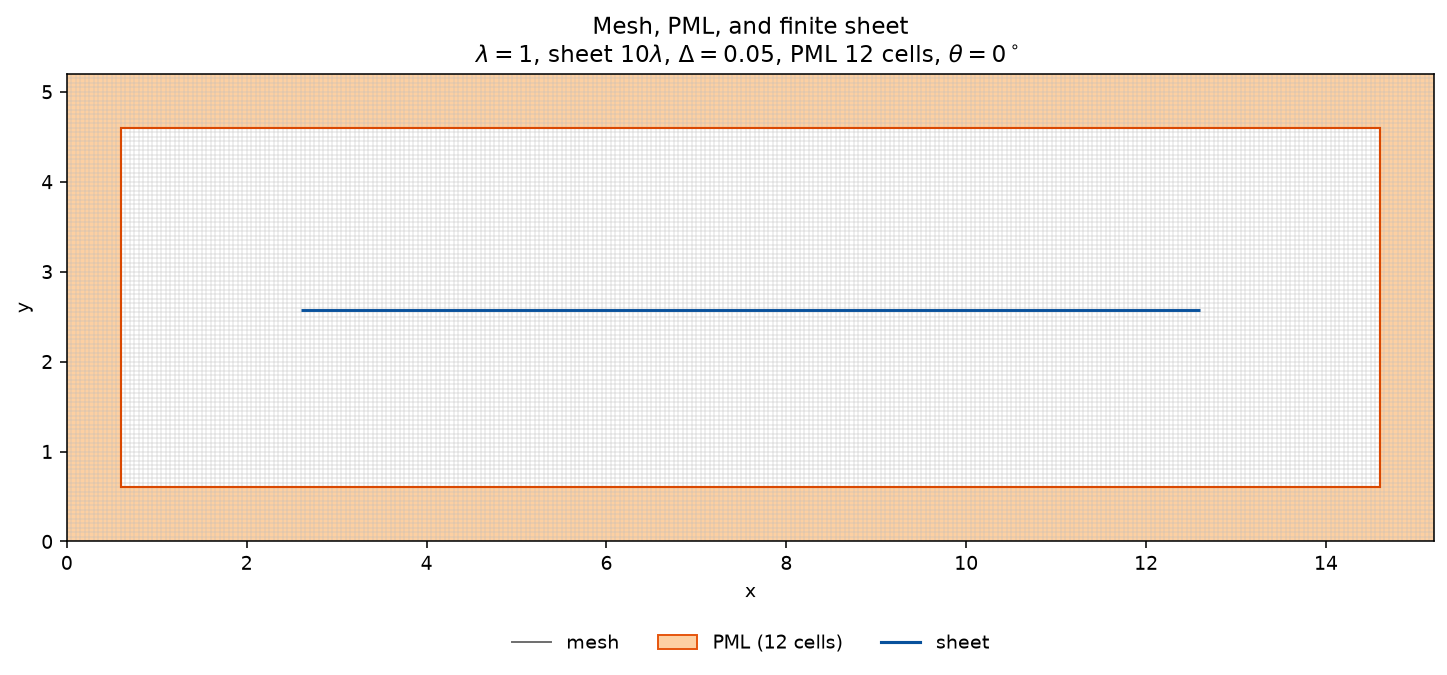
\includegraphics[width=\textwidth]{../examples/fdfd/2d/finite_sheet_lam1_points20_theta0_pml12_sheet10/domain.png}
\caption{Default finite-sheet domain. The blue segment is the $10\lambda$
sheet on a magnetic face. The orange frame is the PML band on all four
sides. The wall behind that band is PEC.}
\label{fig:finite-domain}
\end{figure}

\begin{figure}[ht]
\centering
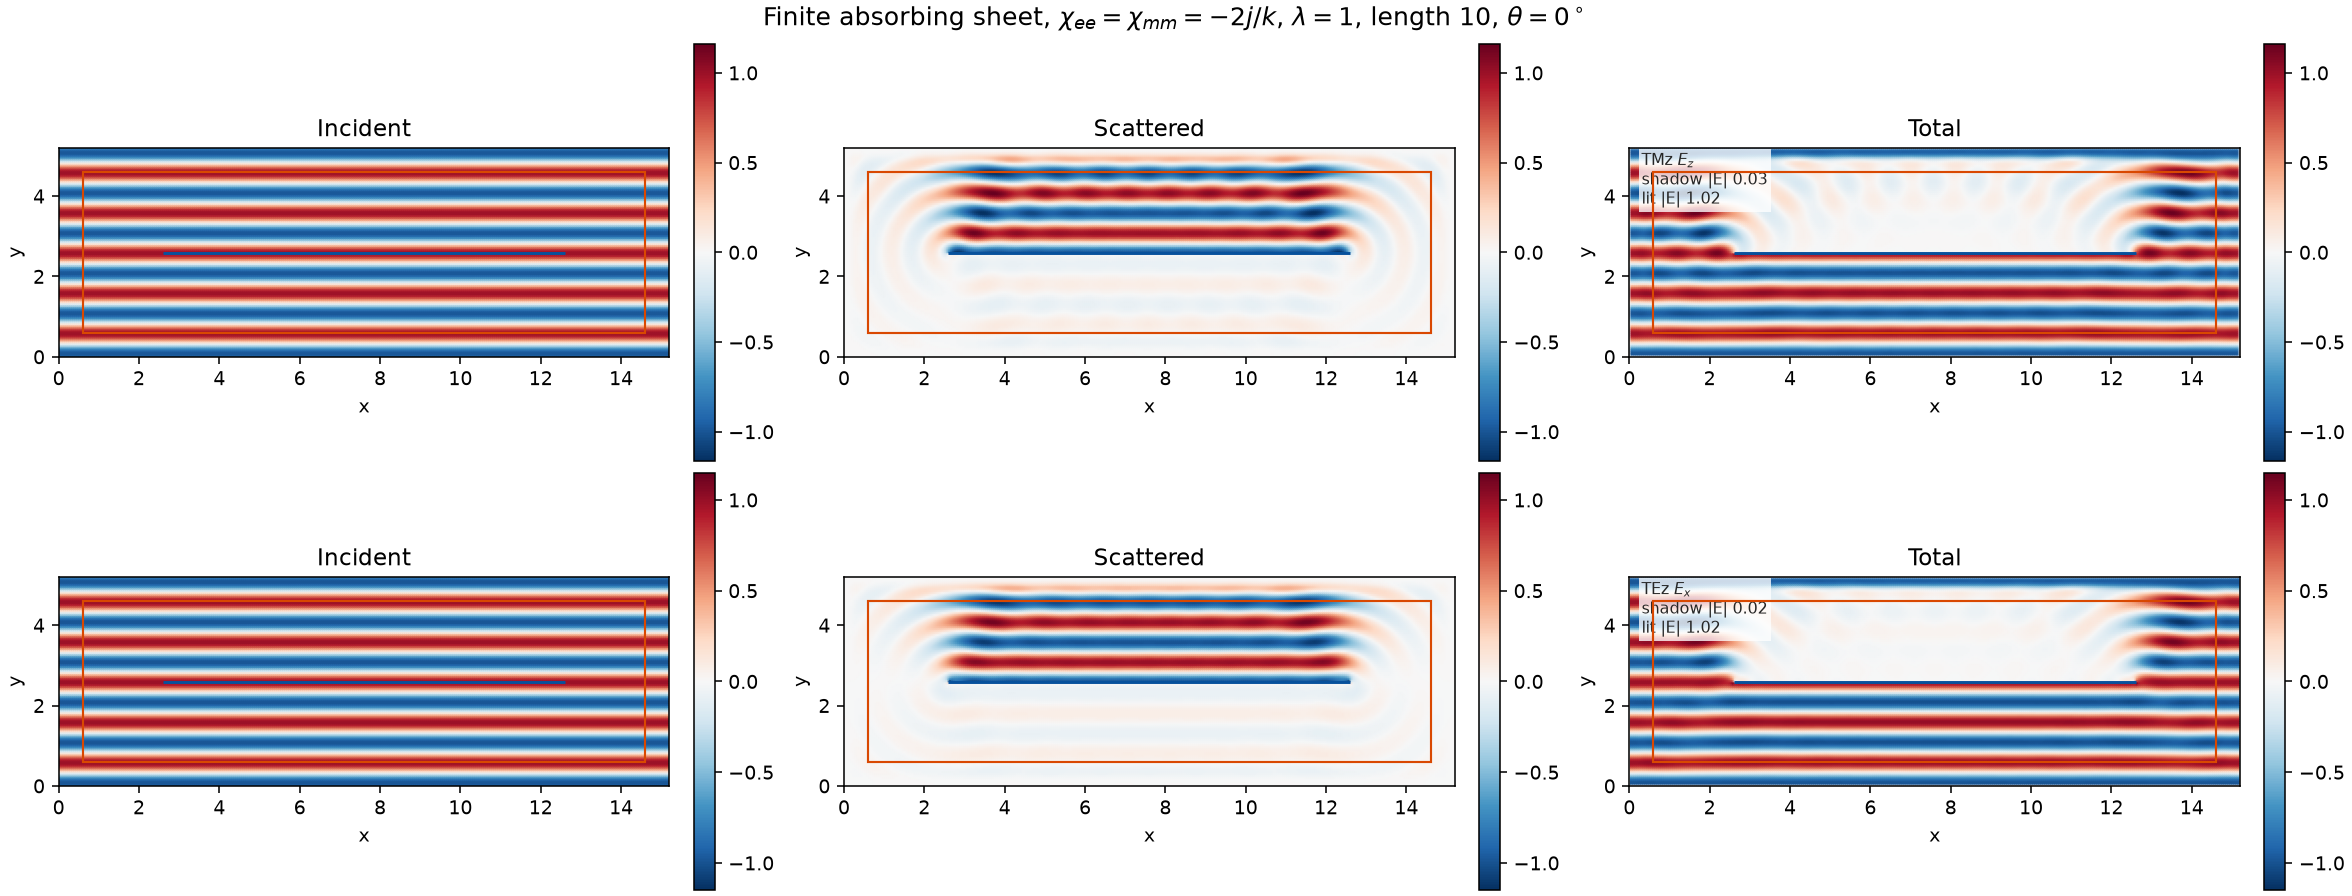
\includegraphics[width=\textwidth]{../examples/fdfd/2d/finite_sheet_lam1_points20_theta0_pml12_sheet10/finite_sheet.png}
\caption{Finite absorbing sheet, $\chi_{ee}=\chi_{mm}=-2j/k$, $\lambda=1$,
length $10\lambda$, $\theta=0$, at $20$ cells per wavelength with $12$ PML
cells on each side. The rows are $\mathrm{Re}\,E_z$ (TMz) and
$\mathrm{Re}\,E_x$ (TEz). The columns are the incident wave, the scattered
field, and the total field. The annotated means are the lit side and the
shadow over the central $6\lambda$ of the sheet.}
\label{fig:finite-fields}
\end{figure}

The same absorber at $30^\circ$ is
\begin{verbatim}
python examples/fdfd/2d/finite_sheet.py --theta 30
\end{verbatim}
and writes
\begin{center}
\path{finite_sheet_lam1_points20_theta30_pml12_sheet10/}.
\end{center}
The susceptibilities are still the normal-incidence pair
$\chi_{ee}=\chi_{mm}=-2j/k$. On this grid the annotated means are a
lit-side $|E|$ of $1.02$ and a shadow $|E|$ of $0.04$ (TMz), and $0.86$
and $0.01$ (TEz). The lit TEz value follows $\cos 30^\circ$ because the
plotted component is $E_x$.

\begin{figure}[ht]
\centering
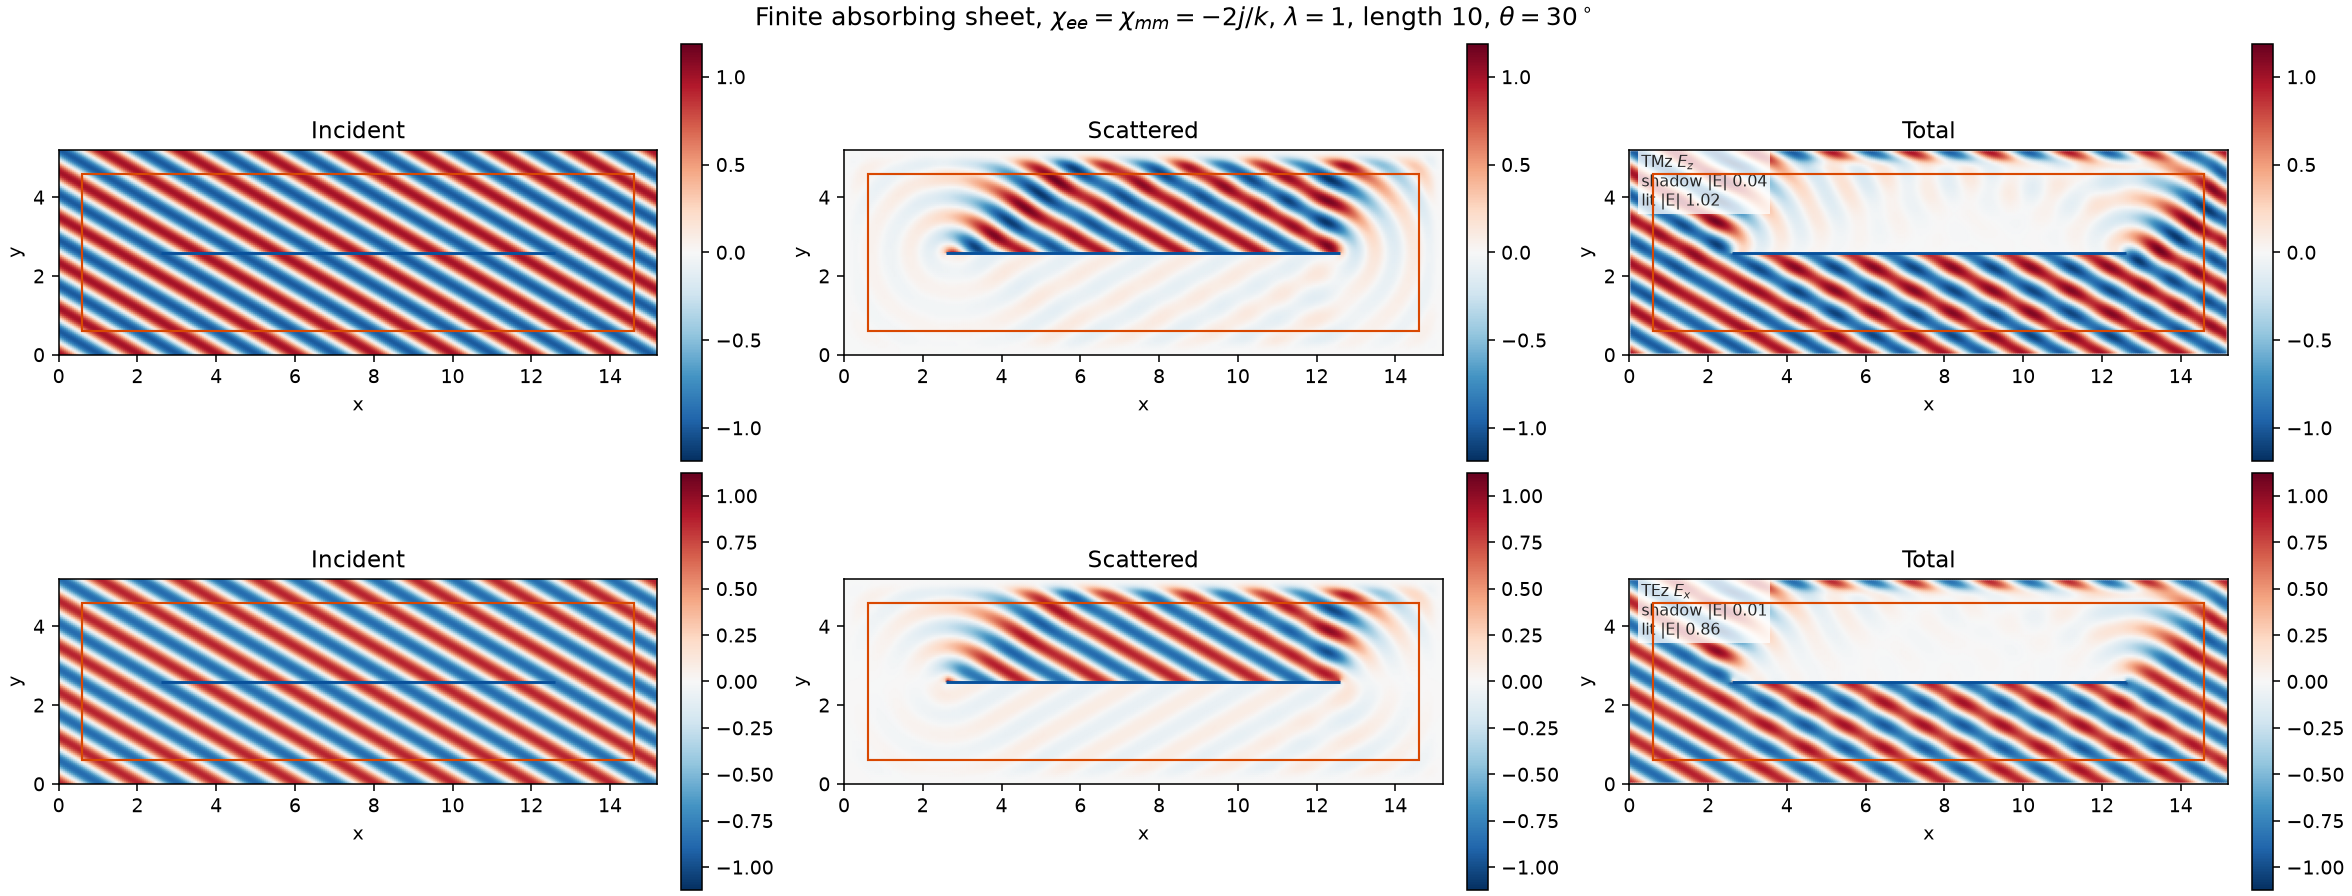
\includegraphics[width=\textwidth]{../examples/fdfd/2d/finite_sheet_lam1_points20_theta30_pml12_sheet10/finite_sheet.png}
\caption{Finite absorbing sheet at $\theta=30^\circ$, with
$\chi_{ee}=\chi_{mm}=-2j/k$, $\lambda=1$, and length $10\lambda$. The
rows are $\mathrm{Re}\,E_z$ (TMz) and $\mathrm{Re}\,E_x$ (TEz). The
annotated means are the lit side and the shadow over the central
$6\lambda$ of the sheet.}
\label{fig:finite-theta}
\end{figure}

\clearpage
\subsection{Periodic oblique sheet}
\label{sec:ex-periodic}

\begin{verbatim}
python examples/fdfd/2d/periodic_sheet.py
\end{verbatim}

\texttt{--chi-ee}, \texttt{--chi-mm}, and \texttt{--chi-nn} are the
tangential electric susceptibility, the tangential magnetic
susceptibility, and the normal magnetic susceptibility. The defaults are
$0.5$, $0.25$, and $0.4$. \texttt{--theta} is the incidence angle in
degrees, measured from the sheet normal, and the default is $30$.
\texttt{--wavelength}, \texttt{--points}, and \texttt{--height} are the
free-space wavelength, the cells per wavelength, and the domain height in
wavelengths. The defaults are $1$, $20$, and $4$.
\texttt{--chi-em} and \texttt{--chi-me} are the magneto-electric
strengths. They default to zero, and a zero stays out of the folder
name. Section~\ref{sec:ex-periodic-cross} sets both to $0.2$.

The sheet spans the whole magnetic face, half a cell below mid-height.
The width is one transverse period, $\lambda/\sin\theta$, so the phase of
an oblique wave closes under a periodic identification of phase one.
\texttt{Boundary.PERIODIC\_X} is that identification in $x$ and a PEC wall
in $y$. The $y$ ends carry the analytic total field. $\chi_{mm}^{nn}$
adds $\chi_{mm}^{nn}\partial_x H_{y,\mathrm{av}}$ on the TMz jump. The
derivative uses the bulk $H_y$, recovered from $E_z$. TEz keeps the
tangential pair, so its reflection and transmission follow $\chi_{ee}$
and $\chi_{mm}$.

The default run writes
\begin{center}
\path{periodic_sheet_lam1_theta30_points20_height4_chiee0.5_chimm0.25_chinn0.4/}
\end{center}
with \texttt{domain.png} and \texttt{periodic\_sheet.png}. At $30^\circ$
the cell is $2\lambda$ wide and $4\lambda$ tall, a $40\times 80$ grid at
$\Delta=0.05$. The field figure shows $\mathrm{Re}\,E_z$ (TMz) and
$\mathrm{Re}\,E_x$ (TEz). The columns are FD, Analytic, and
FD$-$Analytic. On this grid the annotated $L^2$ errors are $9.63\%$
(TMz) and $8.91\%$ (TEz). The regression uses the same susceptibilities
at $10$ cells per wavelength, with the bars $0.24$ and $0.20$.

\begin{figure}[ht]
\centering
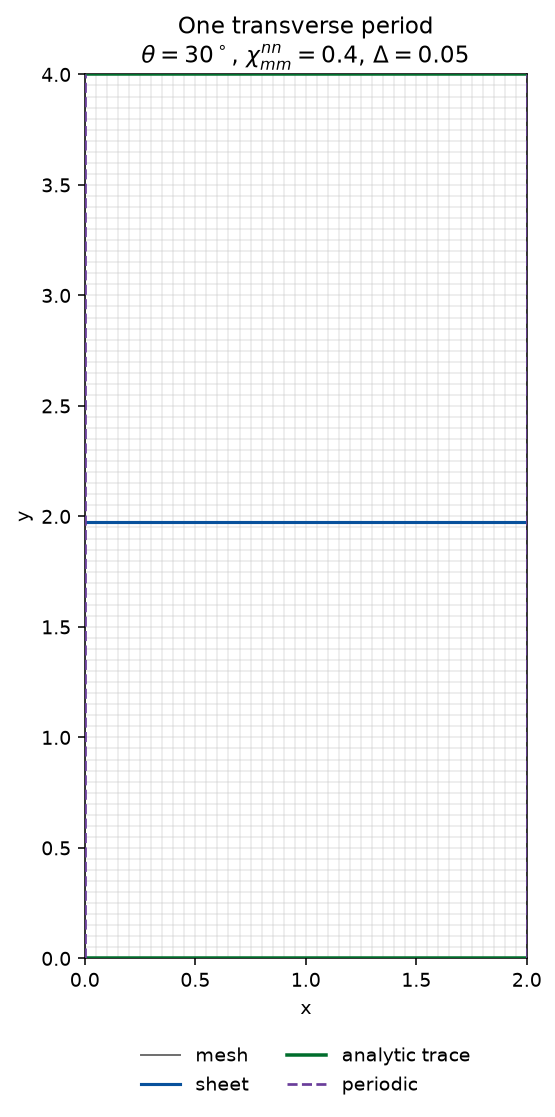
\includegraphics[width=0.48\textwidth]{../examples/fdfd/2d/periodic_sheet_lam1_theta30_points20_height4_chiee0.5_chimm0.25_chinn0.4/domain.png}
\caption{Default periodic-sheet domain. The blue line is the sheet on a
magnetic face. The green lines are the analytic trace on the $y$ ends.
The dashed purple lines mark the periodic identification of the $x$
ends. The width is one transverse period at $30^\circ$.}
\label{fig:periodic-domain}
\end{figure}

\begin{figure}[ht]
\centering
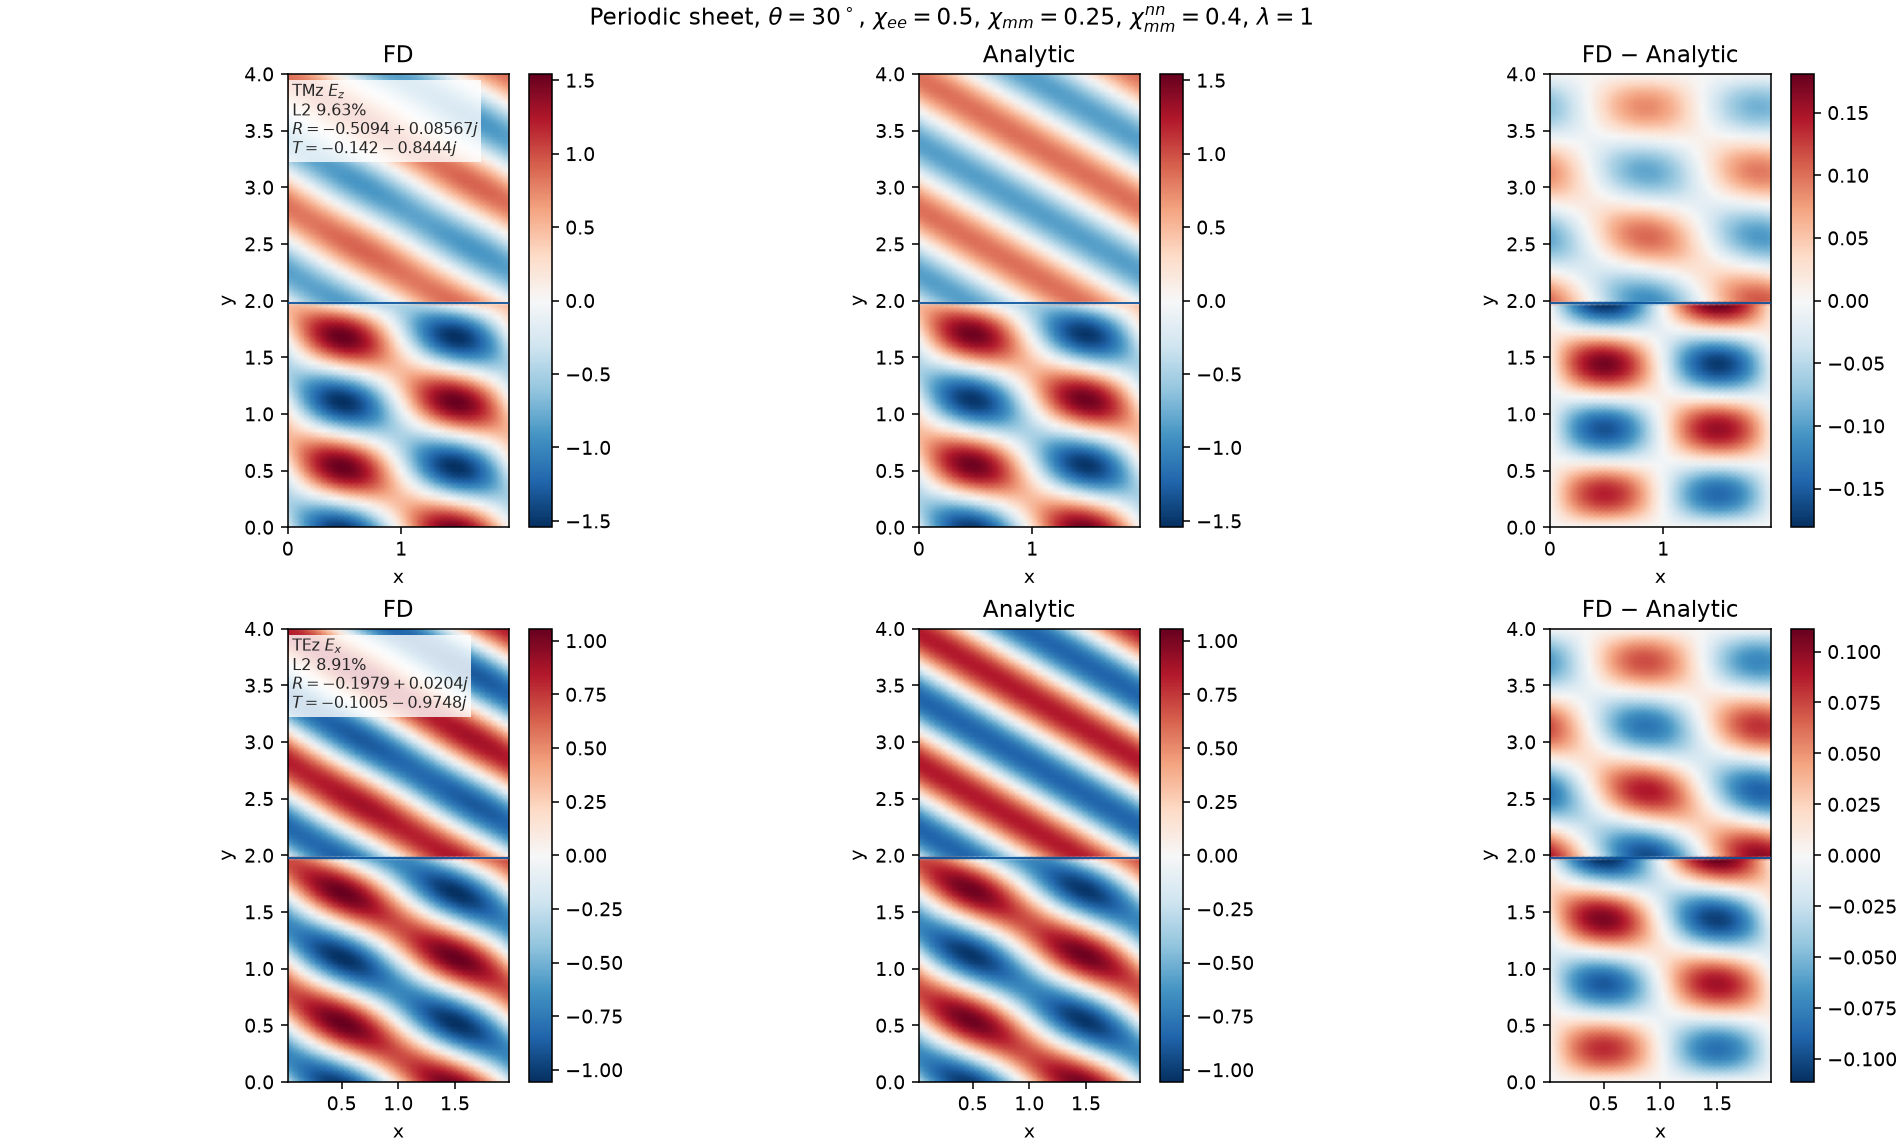
\includegraphics[width=\textwidth]{../examples/fdfd/2d/periodic_sheet_lam1_theta30_points20_height4_chiee0.5_chimm0.25_chinn0.4/periodic_sheet.png}
\caption{Periodic oblique sheet at $\chi_{ee}=0.5$, $\chi_{mm}=0.25$,
$\chi_{mm}^{nn}=0.4$, $\lambda=1$, $\theta=30^\circ$, and a height of
$4\lambda$, on a $40\times 80$ grid at $\Delta=0.05$. The rows are
$\mathrm{Re}\,E_z$ (TMz) and $\mathrm{Re}\,E_x$ (TEz). The columns are
the Yee field, the analytic field, and their difference. The annotated
$L^2$ is the packed free electric vector.}
\label{fig:periodic-fields}
\end{figure}

\clearpage
\subsection{Finite oblique sheet}
\label{sec:ex-finite-oblique}

\begin{verbatim}
python examples/fdfd/2d/finite_sheet.py \
    --chi-ee 0.5 --chi-mm 0.25 --chi-nn 0.4 --theta 30
\end{verbatim}

The geometry is the $10\lambda$ sheet of Sec.~\ref{sec:ex-finite}: $20$
cells per wavelength, $12$ PML cells on each side, and two wavelengths of
vacuum between the sheet and the band. The susceptibilities are the ones
in Sec.~\ref{sec:ex-periodic}, and the incidence is $30^\circ$. The
unknown is the scattered field. The angle enters through the incident
phase. On the TMz jump, $\chi_{mm}^{nn}$ also adds
$\chi_{mm}^{nn}\partial_x H_{y,\mathrm{av}}$. TEz keeps the tangential
pair. A uniform sheet with these values has
$R=-0.5094+0.08567j$ and $T=-0.1420-0.8444j$ in TMz, and
$R=-0.1979+0.02040j$ and $T=-0.1005-0.9748j$ in TEz.

The run writes
\begin{center}
\path{finite_sheet_lam1_points20_theta30_pml12_sheet10_chiee0.5_chimm0.25_chinn0.4/}
\end{center}
with \texttt{domain.png} and \texttt{finite\_sheet.png}. The field figure
shows $\mathrm{Re}\,E_z$ (TMz) and $\mathrm{Re}\,E_x$ (TEz). The columns
are the incident wave, the scattered field, and the total field. On this
grid the annotated means, over the central $6\lambda$ of the sheet, are a
lit-side $|E|$ of $1.15$ and a shadow $|E|$ of $0.85$ (TMz), and $0.90$
and $0.84$ (TEz). A uniform sheet transmits $|E_z|=0.86$ and
$|E_x|=0.85$. The shadow of the finite sheet sits on those values, and
the ends diffract.

\begin{figure}[ht]
\centering
\includegraphics[width=\textwidth]{../examples/fdfd/2d/finite_sheet_lam1_points20_theta30_pml12_sheet10_chiee0.5_chimm0.25_chinn0.4/domain.png}
\caption{Finite oblique-sheet domain. The blue segment is the $10\lambda$
sheet on a magnetic face. The orange frame is the PML band on all four
sides. The incidence is $30^\circ$ and the susceptibilities are
$\chi_{ee}=0.5$, $\chi_{mm}=0.25$, $\chi_{mm}^{nn}=0.4$.}
\label{fig:finite-oblique-domain}
\end{figure}

\begin{figure}[ht]
\centering
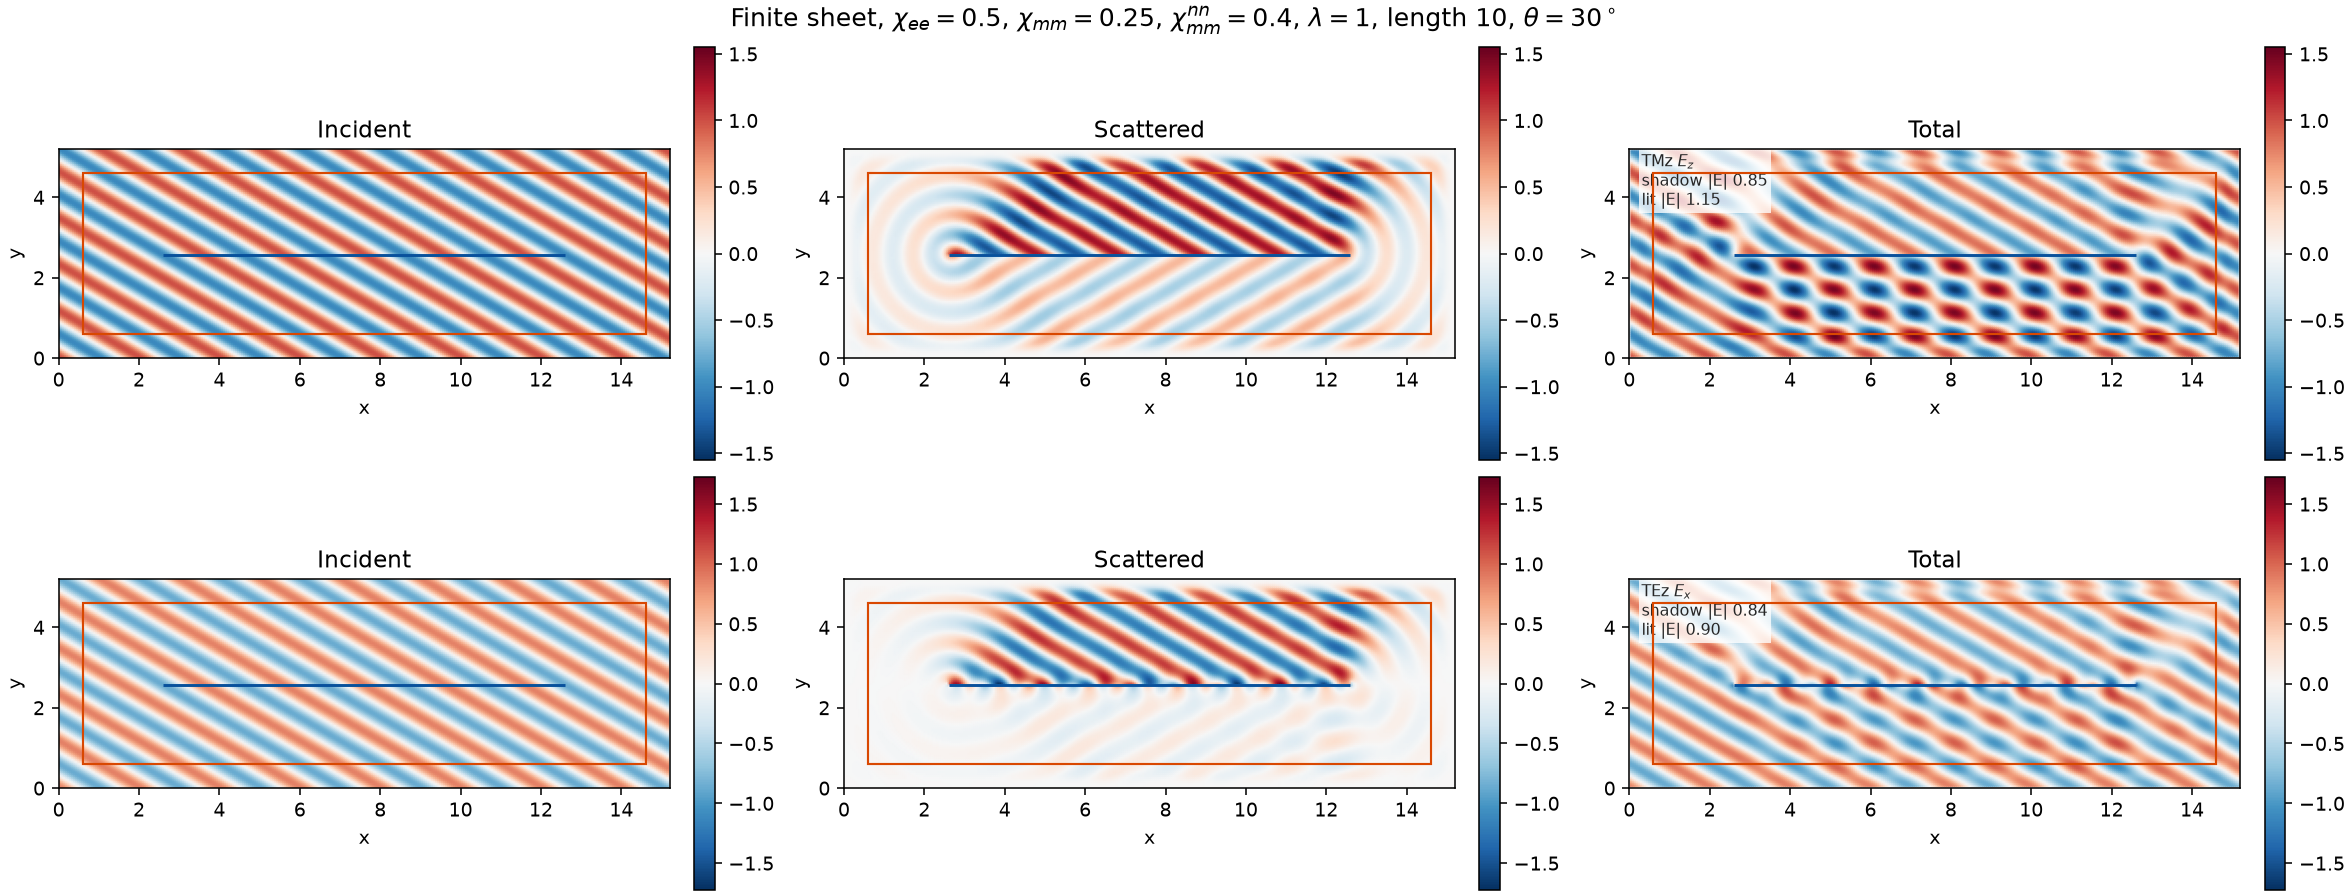
\includegraphics[width=\textwidth]{../examples/fdfd/2d/finite_sheet_lam1_points20_theta30_pml12_sheet10_chiee0.5_chimm0.25_chinn0.4/finite_sheet.png}
\caption{Finite sheet at $\chi_{ee}=0.5$, $\chi_{mm}=0.25$,
$\chi_{mm}^{nn}=0.4$, $\lambda=1$, length $10\lambda$, $\theta=30^\circ$,
at $20$ cells per wavelength with $12$ PML cells on each side. The rows
are $\mathrm{Re}\,E_z$ (TMz) and $\mathrm{Re}\,E_x$ (TEz). The columns
are the incident wave, the scattered field, and the total field. The
annotated means are the lit side and the shadow over the central
$6\lambda$ of the sheet.}
\label{fig:finite-oblique-fields}
\end{figure}

\clearpage
\subsection{Periodic magneto-electric sheet}
\label{sec:ex-periodic-cross}

\begin{verbatim}
python examples/fdfd/2d/periodic_sheet.py --chi-em 0.2 --chi-me 0.2
\end{verbatim}

The geometry and the tangential susceptibilities are those of
Sec.~\ref{sec:ex-periodic}. $\chi_{em}=\chi_{me}=0.2$ is the reciprocal
magneto-electric pair, and both polarizations carry it.
$\chi_{mm}^{nn}$ remains on the TMz jump. A uniform sheet with these
values has $R=-0.07672+0.02351j$ and $T=-0.2819-0.9201j$ in TMz, and
$R=0.329-0.09119j$ and $T=-0.2984-1.077j$ in TEz. The reflective lock
$\chi_{em}=\chi_{me}=-2j/k$, with the other susceptibilities zero, gives
$R=1$ and $T=0$ at normal incidence.

The run writes
\begin{center}
\path{periodic_sheet_lam1_theta30_points20_height4_chiee0.5_chimm0.25_chinn0.4_chiem0.2_chime0.2/}
\end{center}
with \texttt{domain.png} and \texttt{periodic\_sheet.png}. The cell is
again $2\lambda$ wide and $4\lambda$ tall, a $40\times 80$ grid at
$\Delta=0.05$. The field figure shows $\mathrm{Re}\,E_z$ (TMz) and
$\mathrm{Re}\,E_x$ (TEz). The columns are FD, Analytic, and
FD$-$Analytic. On this grid the annotated $L^2$ errors are $8.38\%$
(TMz) and $7.62\%$ (TEz). The regression uses the same susceptibilities
at $10$ cells per wavelength, with the bars $0.24$ and $0.21$.

\begin{figure}[ht]
\centering
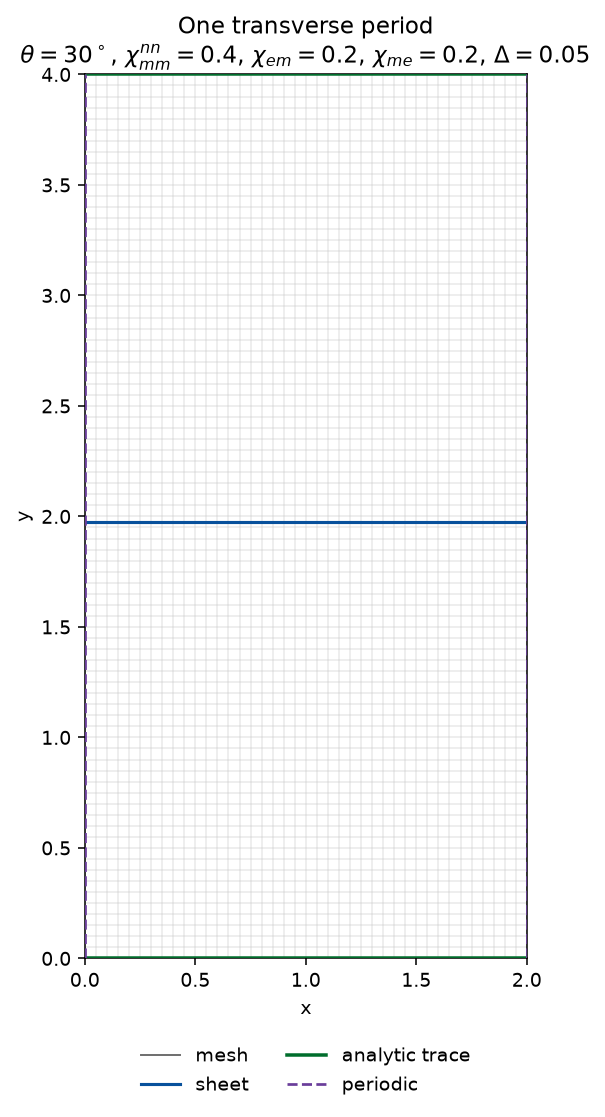
\includegraphics[width=0.48\textwidth]{../examples/fdfd/2d/periodic_sheet_lam1_theta30_points20_height4_chiee0.5_chimm0.25_chinn0.4_chiem0.2_chime0.2/domain.png}
\caption{Periodic magneto-electric domain. The blue line is the sheet on
a magnetic face. The green lines are the analytic trace on the $y$ ends.
The dashed purple lines mark the periodic identification of the $x$
ends. The susceptibilities add $\chi_{em}=\chi_{me}=0.2$ to the
tangential and normal values of Figure~\ref{fig:periodic-domain}.}
\label{fig:periodic-cross-domain}
\end{figure}

\begin{figure}[ht]
\centering
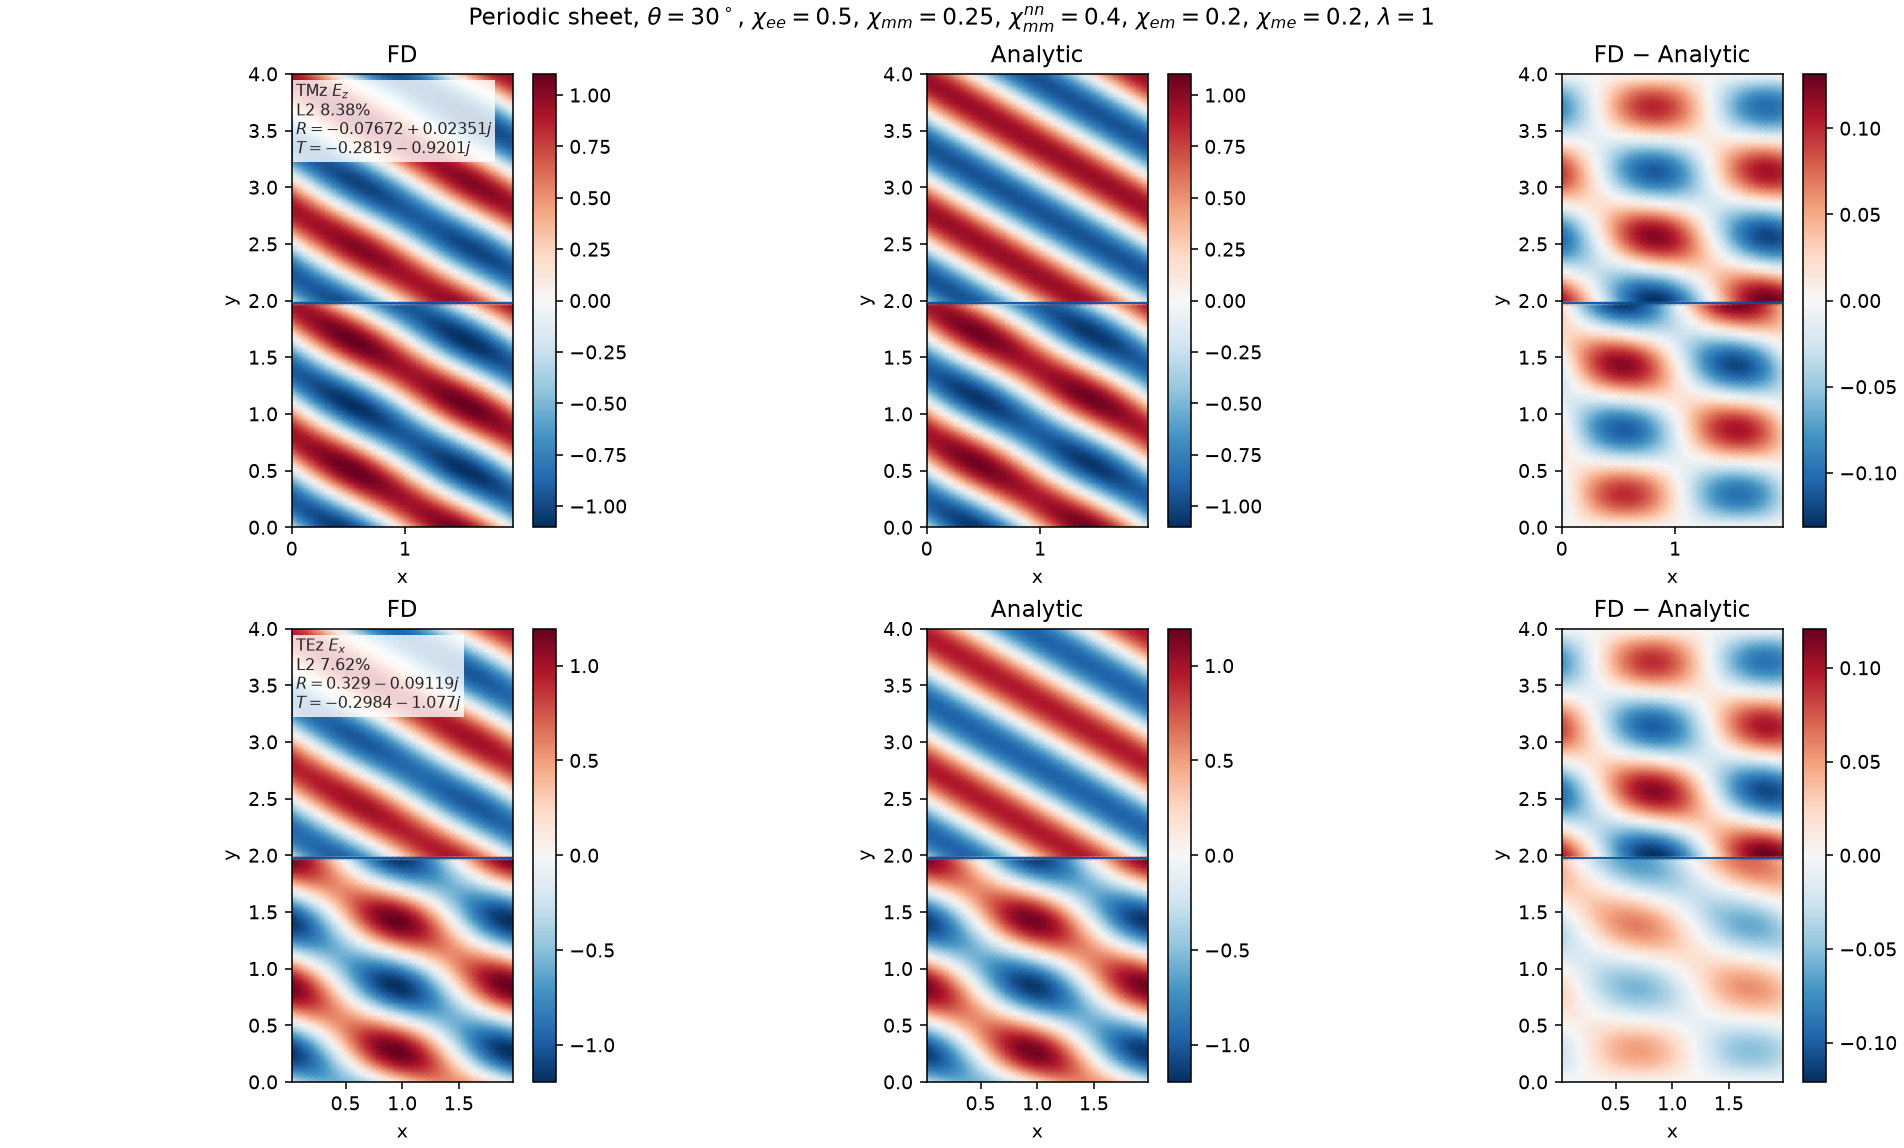
\includegraphics[width=\textwidth]{../examples/fdfd/2d/periodic_sheet_lam1_theta30_points20_height4_chiee0.5_chimm0.25_chinn0.4_chiem0.2_chime0.2/periodic_sheet.png}
\caption{Periodic oblique sheet at $\chi_{ee}=0.5$, $\chi_{mm}=0.25$,
$\chi_{mm}^{nn}=0.4$, $\chi_{em}=\chi_{me}=0.2$, $\lambda=1$,
$\theta=30^\circ$, and a height of $4\lambda$, on a $40\times 80$ grid
at $\Delta=0.05$. The rows are $\mathrm{Re}\,E_z$ (TMz) and
$\mathrm{Re}\,E_x$ (TEz). The columns are the Yee field, the analytic
field, and their difference. The annotated $L^2$ is the packed free
electric vector.}
\label{fig:periodic-cross-fields}
\end{figure}

\clearpage
\subsection{Finite magneto-electric sheet}
\label{sec:ex-finite-cross}

\begin{verbatim}
python examples/fdfd/2d/finite_sheet.py \
    --chi-ee 0.5 --chi-mm 0.25 --chi-nn 0.4 \
    --chi-em 0.2 --chi-me 0.2 --theta 30
\end{verbatim}

The geometry is the $10\lambda$ sheet of Sec.~\ref{sec:ex-finite}: $20$
cells per wavelength, $12$ PML cells on each side, and two wavelengths of
vacuum between the sheet and the band. The susceptibilities and the
incidence are those of Sec.~\ref{sec:ex-periodic-cross}. The unknown is
the scattered field. A uniform sheet transmits $|E_z|=0.96$ and
$|E_x|=0.97$.

The run writes
\begin{center}
\path{finite_sheet_lam1_points20_theta30_pml12_sheet10_chiee0.5_chimm0.25_chinn0.4_chiem0.2_chime0.2/}
\end{center}
with \texttt{domain.png} and \texttt{finite\_sheet.png}. The field figure
shows $\mathrm{Re}\,E_z$ (TMz) and $\mathrm{Re}\,E_x$ (TEz). The columns
are the incident wave, the scattered field, and the total field. On this
grid the annotated means, over the central $6\lambda$ of the sheet, are a
lit-side $|E|$ of $1.01$ and a shadow $|E|$ of $0.97$ (TMz), and $0.85$
and $0.96$ (TEz). The shadow sits on the uniform transmission, and the
ends diffract.

\begin{figure}[ht]
\centering
\includegraphics[width=\textwidth]{../examples/fdfd/2d/finite_sheet_lam1_points20_theta30_pml12_sheet10_chiee0.5_chimm0.25_chinn0.4_chiem0.2_chime0.2/domain.png}
\caption{Finite magneto-electric domain. The blue segment is the
$10\lambda$ sheet on a magnetic face. The orange frame is the PML band
on all four sides. The incidence is $30^\circ$ and the susceptibilities
add $\chi_{em}=\chi_{me}=0.2$ to the values of
Figure~\ref{fig:finite-oblique-domain}.}
\label{fig:finite-cross-domain}
\end{figure}

\begin{figure}[ht]
\centering
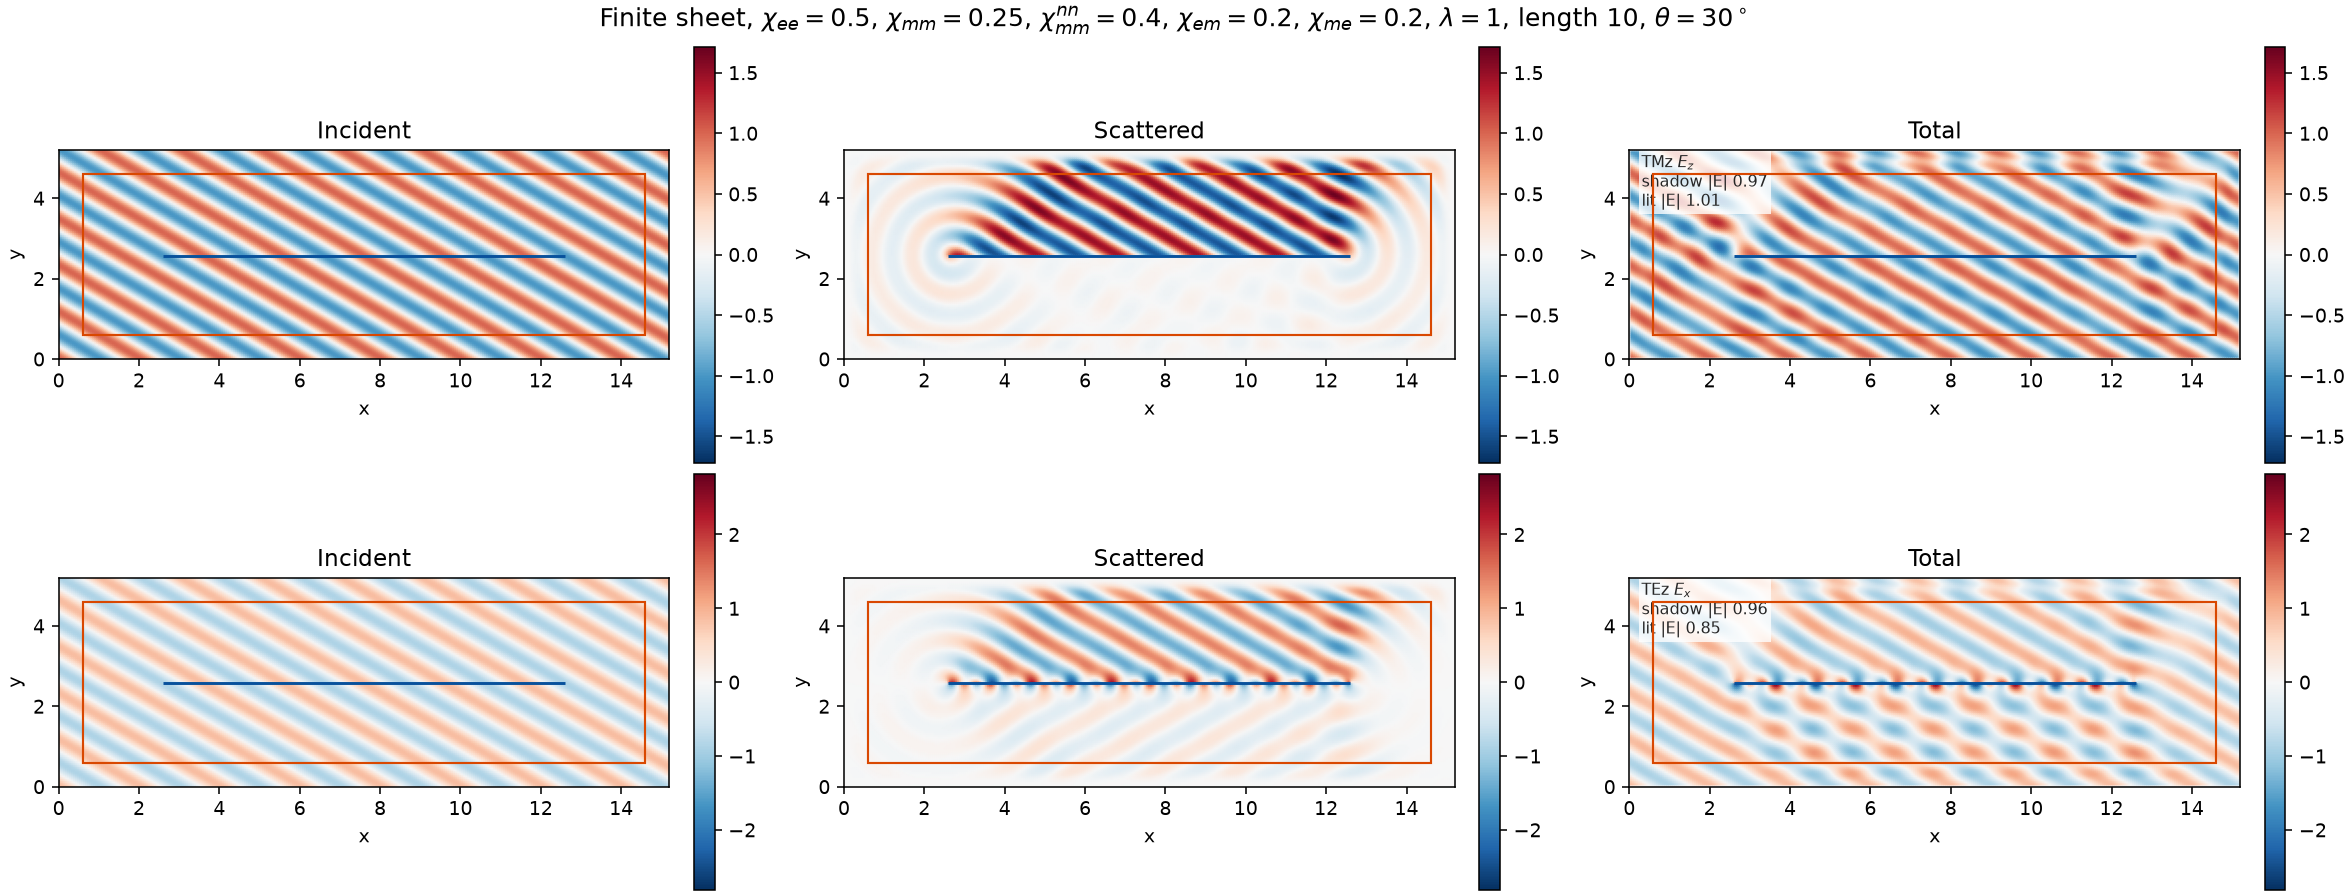
\includegraphics[width=\textwidth]{../examples/fdfd/2d/finite_sheet_lam1_points20_theta30_pml12_sheet10_chiee0.5_chimm0.25_chinn0.4_chiem0.2_chime0.2/finite_sheet.png}
\caption{Finite sheet at $\chi_{ee}=0.5$, $\chi_{mm}=0.25$,
$\chi_{mm}^{nn}=0.4$, $\chi_{em}=\chi_{me}=0.2$, $\lambda=1$, length
$10\lambda$, $\theta=30^\circ$, at $20$ cells per wavelength with $12$
PML cells on each side. The rows are $\mathrm{Re}\,E_z$ (TMz) and
$\mathrm{Re}\,E_x$ (TEz). The columns are the incident wave, the
scattered field, and the total field. The annotated means are the lit
side and the shadow over the central $6\lambda$ of the sheet.}
\label{fig:finite-cross-fields}
\end{figure}

\clearpage
\section{Tests and later slices}
\label{sec:tests}

The suite is \texttt{pytest} from the project root, eighty-four tests in
\texttt{tests/}. Milestone~1 checks the curls, the adjoint, the cavity
eigenvalues, the manufactured solve, the invariant and the CFL growth, and
the fully discrete dispersion, with relative or absolute bars from
$10^{-12}$ to $10^{-6}$ as listed in the formulation note. Milestone~2 adds
the manufactured solve with $\sigma>0$ and with a smooth
$\varepsilon(x,y)$, a uniform $\varepsilon_r=4$ cavity, the slab-loaded
cavity, the lossless staircase invariant, Fresnel face continuity, the Mie
continuity and PEC coefficient, the Fresnel and cylinder $L^2$ bars of
$2\times 10^{-2}$, and one period of Debye and Lorentz evolution. The PML
tests check the grading, the stretched curls, a zero-thickness step, the
line current, and the leapfrog phasor. The formulation note records those
bars: a coarse interior error below $4\times 10^{-2}$, a $2.5\times$ drop
when the spacing is halved on the same physical band, a bare PEC window
above $0.5$, and a phasor error below $1.5\times 10^{-2}$ at $48$ steps
per period. The conductor tests compare a PEC band with the shorter cavity
it leaves, a PMC quarter-wave with the sine formula, and an open PEC
cylinder with the Mie series. The eigenvalue bars are $10^{-10}$. The
open PEC bars are $8\times 10^{-2}$ (TMz) and $10^{-1}$ (TEz), on the
$64^2$ grid of Sec.~\ref{sec:ex-pec}. The open dielectric bars, at
$n=1.5$ on that same grid, are $8\times 10^{-3}$ (TMz) and
$1.3\times 10^{-2}$ (TEz). That comparison keeps the unstretched samples
at least $2\Delta$ off the rim, inside and outside the disk. The 3D
curl bars are $10^{-12}$. On an $8\times 6\times 5$ PEC box the three
pure modes match the semi-discrete frequency, with the $z$ term included,
to $10^{-10}$. A manufactured solve on a $6\times 5\times 4$ box recovers
the electric vector to the same bar. The stretched 3D curls match the
array form to $10^{-12}$ on that box. The 3D Mie series is continuous
across the sphere surface to $10^{-8}$. The open dielectric sphere, at
$n=1.5$ on an $18^3$ box with a PML of $3$ cells, stays under
$1.8\times 10^{-2}$. The Hertzian dipole, with $I\ell=1$ on a $16^3$
box at $\Delta=0.1$, $\lambda=1$, and a PML of $3$ cells, stays under
$0.16$ outside the band and at least $0.25\lambda$ from the element.
The resistive sheet, at $Z_s=\eta_0$ on an
$8\times 80$ box with $\Delta=1$, $\lambda=46$, and the sheet on the
electric node $y=40$, stays under $6\times 10^{-4}$ (TMz, $E_z$) and
$1.2\times 10^{-2}$ (TEz, $E_x$ and $E_y$). The symmetric sheet, on that
box with the face $y=40.5$, $\chi_{ee}=0.5$, and $\chi_{mm}=0.25$, stays
under $4.2\times 10^{-2}$ (TMz) and $1.9\times 10^{-1}$ (TEz). A cell of
$\Delta=1/3$ on the same face drops both errors by more than half. A finite
sheet whose samples stay outside the PML is accepted, and a sheet that
enters the band is refused. On a $4\lambda$ absorber at $10$ cells per
wavelength, with $\chi_{ee}=\chi_{mm}=-2j/k$ and $\theta=0$, the lit-side
mean $|E|$ stays above $0.95$ and the shadow mean stays under $0.20$, in
both polarizations. The $10\lambda$ figure is the example in
Sec.~\ref{sec:ex-finite}. The normal susceptibility, on a periodic cell
one transverse period wide at $30^\circ$, with $\chi_{ee}=0.5$,
$\chi_{mm}=0.25$, $\chi_{mm}^{nn}=0.4$, and a height of $4\lambda$, stays
under $0.24$ (TMz) and $0.20$ (TEz) at $10$ cells per wavelength. Four
times that resolution drops both errors by more than half. With the
tangential susceptibilities at zero and $\chi_{mm}^{nn}=0.4$, the TMz
error at $20$ cells per wavelength stays under $0.17$. The example in
Sec.~\ref{sec:ex-periodic} annotates $9.63\%$ and $8.91\%$ at $20$ cells
per wavelength. The $10\lambda$ sheet with those susceptibilities at
$30^\circ$ is the open example in Sec.~\ref{sec:ex-finite-oblique}. Its
lit and shadow means stay with that figure. The magneto-electric pair, on
that same periodic cell with $\chi_{em}=\chi_{me}=0.2$ added to
$\chi_{ee}=0.5$, $\chi_{mm}=0.25$, and $\chi_{mm}^{nn}=0.4$, stays under
$0.24$ (TMz) and $0.21$ (TEz) at $10$ cells per wavelength. Four times
that resolution drops both errors by more than half. With only
$\chi_{em}=\chi_{me}=0.2$, the error at $20$ cells per wavelength stays
under $0.16$ in both polarizations. The example in
Sec.~\ref{sec:ex-periodic-cross} annotates $8.38\%$ and $7.62\%$ at $20$
cells per wavelength. The $10\lambda$ sheet with those susceptibilities
at $30^\circ$ is the open example in Sec.~\ref{sec:ex-finite-cross}. A failing
bar is a reason to refine the grid in that test, not to widen the bar.

The formulation note already fixes the formulas for the slices that remain
to be coded: impressed beams, a near-to-far
integral, and a Bloch phase. The Fresnel
and dielectric-cylinder domain figures still draw an orange thickness as
a layout. Those two solves use the Dirichlet trace. The open PEC cylinder
of Sec.~\ref{sec:ex-pec}, the open dielectric cylinder of
Sec.~\ref{sec:ex-diel}, the open dielectric sphere of
Sec.~\ref{sec:ex-sphere}, the Hertzian dipole of
Sec.~\ref{sec:ex-dipole}, the finite absorbing sheet of
Sec.~\ref{sec:ex-finite}, the finite oblique sheet of
Sec.~\ref{sec:ex-finite-oblique}, and the finite magneto-electric sheet of
Sec.~\ref{sec:ex-finite-cross} are the solves that stretch the derivatives.

\clearpage
\begin{thebibliography}{9}
\bibitem{yee1966}
K.~S. Yee, ``Numerical solution of initial boundary value problems
involving Maxwell's equations in isotropic media,'' \emph{IEEE Trans.\
Antennas Propag.}, 1966.
\bibitem{smy2017}
T.~J. Smy, S. Stewart, and S. Gupta, ``Integrated generalized sheet
transition conditions in a Yee-cell based FDTD simulation of
electromagnetic metasurfaces,'' arXiv:1706.10136, 2017.
\end{thebibliography}

\end{document}
